\newpage
\section{Casi d'uso}
Questa sezione elenca le funzionalità offerte da \progetto\ descritte attraverso il linguaggio \gloss{UML}.
\progetto\ può essere visto come l'insieme di più sottosistemi che verranno di seguito elencati e che sono stati descritti in modo molto generale anche attraverso la Figura \ref{fig:butterfly}.\\
Questa mostra la suddivisione di \progetto\ nei sottosistemi in cui è composto e ne facilita l'analisi per la stesura dei casi d'uso.
Abbiamo quindi come attori non soltanto le applicazioni che mandano messaggi al sistema ma anche componente inoltre quali Producer e Consumer che hanno interazioni con il Broker.
	
	\subsection{Attori}
	\begin{itemize}
		\item Redmine/GitLab
		\item Producer
		\item Utente non acceduto
		\item Utente (acceduto), che interagisce col Gestore Personale
		\item Consumer
		\item Telegram/e-mail
	\end{itemize}
	
	\subsection{Elenco casi d'uso}

%TODO: da ricordarsi: se qualcuno è offline, c'è la possibilità che il messaggio venga perso.

\newcounter{uccount}

\stepcounter{uccount}

\subsubsection{UC\theuccount-R - Redmine segnala apertura issue a Producer Redmine}
    \begin{figure}[H]
		\centering
		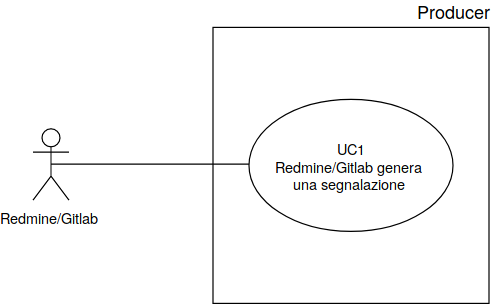
\includegraphics[width=0.7\textwidth]{img/UC1.png}\\
		\caption{UCR\theuccount-R - Redmine segnala apertura issue a Producer
			Redmine}
	\end{figure}
	\begin{itemize}
		\item \textbf{Codice}: UCR\theuccount-R.
		\item \textbf{Titolo}: Redmine segnala apertura issue a Producer Redmine.
		\item \textbf{Attori primari}: Redmine.
		\item \textbf{Descrizione}: il sistema qui è il Producer Redmine ed è interno al sistema \progetto.
		 L'apertura di una issue in un particolare progetto su Redmine
		 contiene i seguenti campi di interesse:
		 \begin{itemize}
		 	\item Tracker
		 	\item Subject
		 	\item Status
		 	\item Priority e opzionalmente:
		 	\begin{itemize}
		 		\item Description
		 		\item Assignee
		 	\end{itemize}
		 \end{itemize}
		\item \textbf{Precondizione}: Viene aperta una issue su Redmine e
		segnalata a \progetto.
		\item \textbf{Postcondizione}: il Producer Redmine riceve la segnalazione da Redmine.
		\item \textbf{Scenario principale}: 
		\begin{enumerate}
			\item Redmine procede all'invio della segnalazione di issue al Producer Redmine.
		\end{enumerate}
		
	\end{itemize}


\stepcounter{uccount}

	\subsubsection{UC\theuccount-PR - Gitlab segnala la modifica di una issue al Producer Redmine}
	\begin{figure}[H]
		\centering
		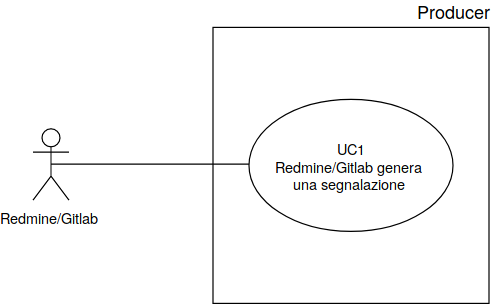
\includegraphics[width=0.7\textwidth]{img/UC1.png}\\
		\caption{UC\theuccount-PR - Redmine segnala la modifica di una issue al Producer Redmine}
	\end{figure}
	\begin{itemize}
		\item \textbf{Codice}: UC\theuccount-PR.
		\item \textbf{Titolo}: Redmine segnala la modifica di una issue al Producer Redmine.
		\item \textbf{Attori primari}: Redmine.
		\item \textbf{Descrizione}: l'invio di una segnalazione avviene
		da parte di Redmine tramite webhook, quando una issue viene modificata.
		\item \textbf{Precondizione}: Viene modificata una issue già aperta su un
		progetto di Redmine e segnalata a \progetto.
		\item \textbf{Postcondizione}: il Producer Redmine riceve la segnalazione da Redmine.
		\item \textbf{Scenario principale}: 
		\begin{enumerate}
			\item Redmine procede all'invio della segnalazione di modifica issue al Producer Redmine.
		\end{enumerate}
		
	\end{itemize}

\stepcounter{uccount}

\subsubsection{UC\theuccount-PG - GitLab segnala apertura issue al Producer GitLab}
	\begin{figure}[H]
		\centering
		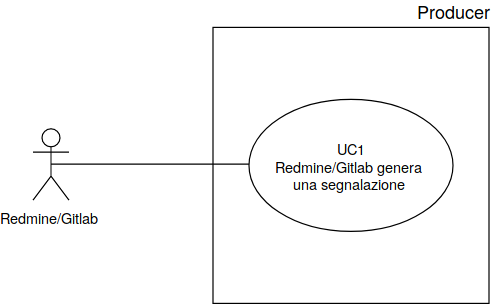
\includegraphics[width=0.7\textwidth]{img/UC1.png}\\
		\caption{UC\theuccount-PG - GitLab segnala apertura issue al Producer GitLab}
	\end{figure}
	\begin{itemize}
		\item \textbf{Codice}: UC\theuccount-PG.
		\item \textbf{Titolo}: GitLab segnala apertura issue al Producer GitLab.
		\item \textbf{Attori primari}: GitLab.
		\item \textbf{Descrizione}: l'invio di
		una segnalazione avviene da parte di GitLab tramite webhook. L'apertura di
		una issue su GitLab contiene:
		\begin{itemize}
			\item Title e opzionalmente:
			\begin{itemize}
				\item Label
				\item Milestone
				\item Assignees
				\item Due Date
			\end{itemize}
		\end{itemize}
		\item \textbf{Precondizione}: Viene aperta una issue su GitLab e 
		segnalata a \progetto.
		\item \textbf{Postcondizione}: il Producer GitLab riceve la segnalazione da GitLab.
		\item \textbf{Scenario principale}: 
		\begin{enumerate}
			\item GitLab procede all'invio della segnalazione di issue al Producer GitLab.
		\end{enumerate}
		
	\end{itemize}

\stepcounter{uccount}

\subsubsection{UC\theuccount-G - GitLab segnala evento di push a Producer GitLab}
	\begin{figure}[H]
		\centering
		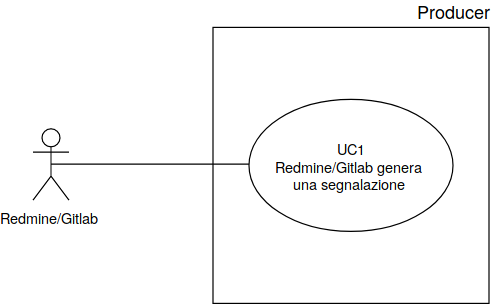
\includegraphics[width=0.7\textwidth]{img/UC1.png}\\
		\caption{UC\theuccount-G - GitLab segnala evento di push a Producer GitLab}
	\end{figure}
	\begin{itemize}
		\item \textbf{Codice}: UC\theuccount-G.
		\item \textbf{Titolo}: GitLab segnala evento di push a Producer GitLab.
		\item \textbf{Attori primari}: GitLab.
		\item \textbf{Descrizione}: l'invio di una segnalazione avviene da parte di GitLab tramite webhook. L'evento di
		push può essere composto da uno o più commit.
		\item \textbf{Precondizione}: Viene effettuato un push su GitLab e segnalato a \progetto.
		\item \textbf{Postcondizione}: il Producer GitLab riceve la segnalazione da GitLab.
		\item \textbf{Scenario principale}: 
		\begin{enumerate}
			\item GitLab procede all'invio della segnalazione di push al Producer GitLab.
		\end{enumerate}
		
	\end{itemize}

\stepcounter{uccount}

\subsubsection{UC\theuccount-PG - GitLab segnala evento di push a Producer GitLab}
	\begin{figure}[H]
		\centering
		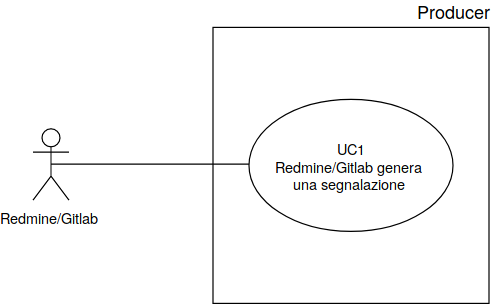
\includegraphics[width=0.7\textwidth]{img/UC1.png}\\
		\caption{UC\theuccount-PG - GitLab segnala evento di push a Producer GitLab}
	\end{figure}
	\begin{itemize}
		\item \textbf{Codice}: UC\theuccount-PG.
		\item \textbf{Titolo}: GitLab segnala evento di push a Producer GitLab.
		\item \textbf{Attori primari}: GitLab.
		\item \textbf{Descrizione}: l'invio di una segnalazione avviene da parte di GitLab tramite webhook. L'evento di
		push può essere composto da uno o più commit.
		\item \textbf{Precondizione}: Viene effettuato un push su GitLab e segnalato a \progetto.
		\item \textbf{Postcondizione}: il Producer GitLab riceve la segnalazione da GitLab.
		\item \textbf{Scenario principale}: 
		\begin{enumerate}
			\item GitLab procede all'invio della segnalazione di push al Producer GitLab.
		\end{enumerate}
		
	\end{itemize}

\stepcounter{uccount}

\subsubsection{UC\theuccount-PGL - Producer GitLab invia messaggio al Gestore Personale}
	\begin{figure}[H]
		\centering
		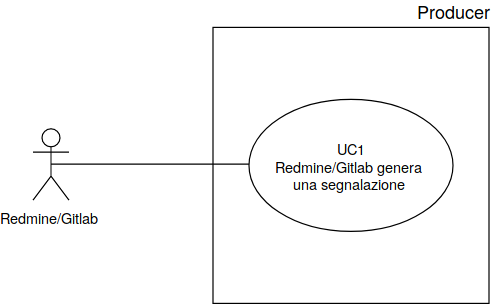
\includegraphics[width=0.7\textwidth]{img/UC1.png}\\
		\caption{UC\theuccount-PGL - Producer GitLab invia messaggio al Gestore Personale}
	\end{figure}
	\begin{itemize}
		\item \textbf{Codice}: UC\theuccount-PGL.
		\item \textbf{Titolo}: Producer GitLab invia messaggio al Gestore Personale.
		\item \textbf{Attori primari}: Producer GitLab.
		\item \textbf{Descrizione}: il sistema qui è Gestore Personale ed è interno al sistema Butterfly. Il Producer GitLab,
		dopo aver ricevuto una segnalazione da GitLab, elabora un messaggio da inviare al Gestore Personale.
		\item \textbf{Precondizione}: il Producer GitLab ha ricevuto una segnalazione da GitLab.
		\item \textbf{Postcondizione}: l Producer GitLab ha inviato al Gestore Personale il messaggio elaborato.
		\item \textbf{Scenario principale}: 
		\begin{enumerate}
			\item Producer GitLab procede all'invio del messaggio al Gestore Personale.
		\end{enumerate}
		
	\end{itemize}
	
	\paragraph{UC\theuccount.1-PGL - Producer GitLab invia uno o più messaggi di commit al Gestore Personale}
	\begin{figure}[H]
		\centering
		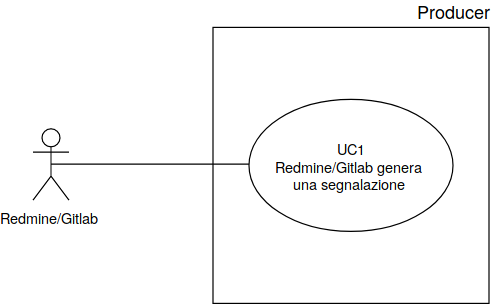
\includegraphics[width=0.7\textwidth]{img/UC1.png}\\
		\caption{UC\theuccount.1-PGL - Producer GitLab invia uno o più messaggi di commit al Gestore Personale}
	\end{figure}
	\begin{itemize}
		\item \textbf{Codice}: UC\theuccount.1-PGL.
		\item \textbf{Titolo}: Producer GitLab invia uno o più messaggi di commit al Gestore Personale.
		\item \textbf{Attori primari}: Producer GitLab.
		\item \textbf{Descrizione}: il sistema qui è Gestore Personale ed è interno al sistema Butterfly. Il Producer GitLab, dopo
		aver ricevuto una segnalazione di push da GitLab, elabora un messaggio per commit che verrà catalogato sotto il Topic "commits".
		Il messaggio elaborato conterrà i campi:
		\begin{itemize}
			\item Project
			\item Topic
			\item Message
		\end{itemize}
		\item \textbf{Precondizione}: il Producer GitLab ha ricevuto una segnalazione da GitLab.
		\item \textbf{Postcondizione}: il Producer GitLab ha inviato uno o più messaggi elaborati di commit.
		\item \textbf{Scenario principale}: 
		\begin{enumerate}
			\item Producer GitLab procede all'invio di uno o più messaggi
		 di commit al Gestore Personale.
		\end{enumerate}
		
	\end{itemize}

	\paragraph{UC\theuccount.2-PGL -  Producer GitLab invia messaggio di issue al Gestore Personale}
	\begin{figure}[H]
		\centering
		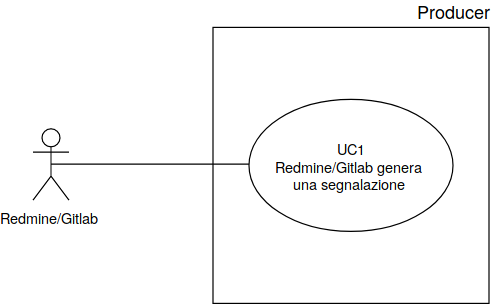
\includegraphics[width=0.7\textwidth]{img/UC1.png}\\
		\caption{UC\theuccount.2-PGL -  Producer GitLab invia messaggio di issue al Gestore Personale}
	\end{figure}
	\begin{itemize}
		\item \textbf{Codice}: UC\theuccount.2-PGL.
		\item \textbf{Titolo}:  Producer GitLab invia messaggio di issue al Gestore Personale.
		\item \textbf{Attori primari}: Producer GitLab.
		\item \textbf{Descrizione}: il sistema qui è Gestore Personale ed è interno al sistema Butterfly. Il Producer GitLab, dopo
		aver ricevuto una segnalazione di issue da GitLab, controlla se la issue è appena stata creata o si tratta di una modifica di
		una issue preesistente. Il messaggio elaborato, una volta elaborato, conterrà i campi:
		\begin{itemize}
			\item Project
			\item Topic
			\item Subject e opzionalmente:
			\begin{itemize}
				\item Description
				\item Due Date
				\item Milestone
				\item Assignee
			\end{itemize}
		\end{itemize}
		\item \textbf{Precondizione}: il Producer GitLab ha ricevuto una segnalazione da GitLab.
		\item \textbf{Postcondizione}: il Producer GitLab ha inviato al Gestore Personale il messaggio \newline elaborato.
		\item \textbf{Scenario principale}: 
		\begin{enumerate}
			\item Producer GitLab procede all'invio di un messaggio di
			issue al Gestore Personale.
		\end{enumerate}
		
	\end{itemize}
	
		\subparagraph{UC\theuccount.2.1-PGL - Producer GitLab invia messaggio di una nuova issue al Gestore Personale}
		\begin{figure}[H]
			\centering
			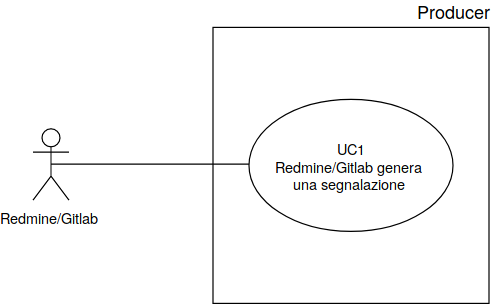
\includegraphics[width=0.7\textwidth]{img/UC1.png}\\
			\caption{UC\theuccount.2.1-PGL - Producer GitLab invia messaggio di una nuova issue al Gestore Personale}
		\end{figure}
		\begin{itemize}
			\item \textbf{Codice}: UC\theuccount.2.1-PGL.
			\item \textbf{Titolo}: Producer GitLab invia messaggio di una nuova issue al Gestore Personale.
			\item \textbf{Attori primari}: Producer GitLab.
			\item \textbf{Descrizione}: il sistema qui è Gestore Personale ed è interno al sistema Butterfly. Il Producer GitLab, dopo
			aver ricevuto una segnalazione di una nuova issue da GitLab, elabora il messaggio che conterrà i campi:
			\begin{itemize}
				\item Project
				\item Topic
				\item Subject e opzionalmente:
				\begin{itemize}
					\item Description
					\item Due Date
					\item Milestone
					\item Assignee
				\end{itemize}
			\end{itemize}
			\item \textbf{Precondizione}: il Producer GitLab ha ricevuto una segnalazione da GitLab.
			\item \textbf{Postcondizione}: il Producer GitLab ha inviato al Gestore Personale il messaggio elaborato di nuova issue.
			\item \textbf{Scenario principale}: 
			\begin{enumerate}
				\item Producer GitLab procede all'invio di un messaggio di
				nuova issue al Gestore Personale.
			\end{enumerate}
			
		\end{itemize}
	
		\subparagraph{UC\theuccount.2.2-PGL - Producer GitLab invia messaggio di modifica di una issue al Gestore Personale}
		\begin{figure}[H]
			\centering
			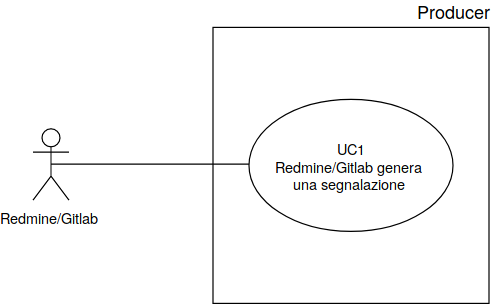
\includegraphics[width=0.7\textwidth]{img/UC1.png}\\
			\caption{UC\theuccount.2.2-PGL - Producer GitLab invia messaggio di modifica di una issue al Gestore Personale}
		\end{figure}
		\begin{itemize}
			\item \textbf{Codice}: UC\theuccount.2.2-PGL.
			\item \textbf{Titolo}: Producer GitLab invia messaggio di modifica di una issue al Gestore Personale.
			\item \textbf{Attori primari}: Producer GitLab.
			\item \textbf{Descrizione}: il sistema qui è Gestore Personale ed è interno al sistema Butterfly. l Producer GitLab, dopo
			aver ricevuto una segnalazione di modifica di una issue da GitLab, controlla se sono stati modificati i campi Label o Title.
			In caso positivo, viene inviato un messaggio elaborato al Gestore Personale, il quale conterrà:
			\begin{itemize}
				\item Project
				\item Topic
				\item Subject e opzionalmente:
				\begin{itemize}
					\item Description
					\item Due Date
					\item Milestone
					\item Assignee
				\end{itemize}
			\end{itemize}
			\item \textbf{Precondizione}: il Producer GitLab ha ricevuto una segnalazione da GitLab.
			\item \textbf{Postcondizione}: il Producer GitLab ha inviato al Gestore Personale il messaggio elaborato di modifica issue.
			\item \textbf{Scenario principale}: 
			\begin{enumerate}
				\item Producer GitLab procede all'invio di un messaggio di modifica issue al Gestore Personale.
			\end{enumerate}
			\item \textbf{Estensioni}: 
			\begin{enumerate}
				\item Ci sono dei messaggi non validi e vengono scartati [UCPGL\theuccount.2.3].
			\end{enumerate}
		\end{itemize}
	
		\subparagraph{UC\theuccount.2.3-PGL - Producer GitLab scarta i messaggi non validi}
		\begin{figure}[H]
			\centering
			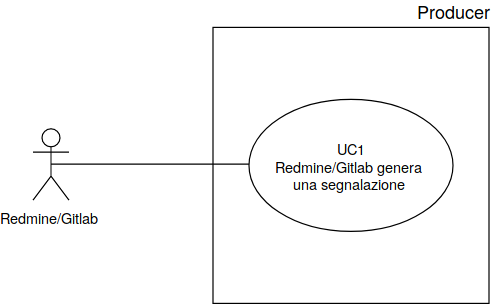
\includegraphics[width=0.7\textwidth]{img/UC1.png}\\
			\caption{UC\theuccount.2.3-PGL - Producer GitLab scarta i messaggi non validi}
		\end{figure}
		\begin{itemize}
			\item \textbf{Codice}: UC\theuccount.2.3-PGL.
			\item \textbf{Titolo}: Producer GitLab scarta i messaggi non validi.
			\item \textbf{Attori primari}: Producer GitLab.
			\item \textbf{Descrizione}: il Producer GitLab, dopo aver ricevuto una segnalazione di una modifica issue da GitLab, controlla
			se sono state modificati i campi Label o Title. In caso negativo, il messaggio viene scartato.
			\item \textbf{Precondizione}: il Producer GitLab ha ricevuto una segnalazione da GitLab.
			\item \textbf{Postcondizione}: il Producer GitLab ha scartato il messaggio.
			\item \textbf{Scenario principale}: 
			\begin{enumerate}
				\item Producer GitLab scarta i messaggi non validi.
			\end{enumerate}
		\end{itemize}

\stepcounter{uccount}

\subsubsection{UC\theuccount-GP - Producer GitLab invia messaggio al Gestore Personale}
	\begin{figure}[H]
		\centering
		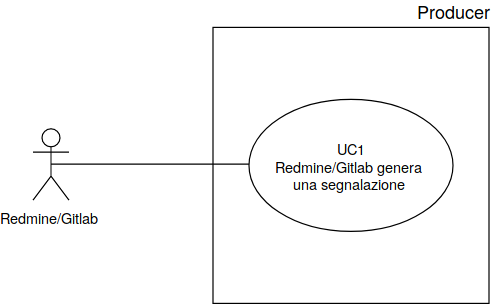
\includegraphics[width=0.7\textwidth]{img/UC1.png}\\
		\caption{UC\theuccount-GP - Producer GitLab invia messaggio al Gestore Personale}
	\end{figure}
	\begin{itemize}
		\item \textbf{Codice}: UC\theuccount-GP.
		\item \textbf{Titolo}: Producer GitLab invia messaggio al Gestore Personale.
		\item \textbf{Attori primari}: Producer GitLab.
		\item \textbf{Descrizione}: il Producer GitLab, dopo aver ricevuto una segnalazione da GitLab, elabora un messaggio da inviare al Gestore Personale.
		\item \textbf{Precondizione}: il Producer GitLab ha ricevuto una segnalazione da GitLab.
		\item \textbf{Postcondizione}: l Producer GitLab ha inviato al Gestore Personale il messaggio elaborato.
		\item \textbf{Scenario principale}: 
		\begin{enumerate}
			\item Producer GitLab procede all'invio del messaggio al Gestore Personale.
		\end{enumerate}
		
	\end{itemize}
	
	\paragraph{UC\theuccount.1-GP - Producer GitLab invia uno o più messaggi di commit al Gestore Personale}
		\begin{figure}[H]
			\centering
			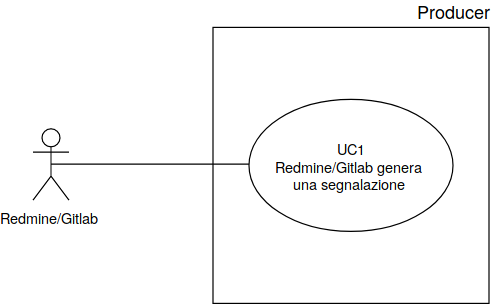
\includegraphics[width=0.7\textwidth]{img/UC1.png}\\
			\caption{UC\theuccount.1-GP - Producer GitLab invia uno o più messaggi di commit al Gestore Personale}
		\end{figure}
		\begin{itemize}
			\item \textbf{Codice}: UC\theuccount.1-GP.
			\item \textbf{Titolo}: Producer GitLab invia uno o più messaggi di commit al Gestore Personale.
			\item \textbf{Attori primari}: Producer GitLab.
			\item \textbf{Descrizione}: il Producer GitLab, dopo aver ricevuto una segnalazione di push da GitLab,
			elabora un messaggio per commit che verrà catalogato sotto il Topic "commits".
			Il messaggio elaborato conterrà i campi:
			\begin{itemize}
				\item Project
				\item Topic
				\item Message
			\end{itemize}
			\item \textbf{Precondizione}: il Producer GitLab ha ricevuto una segnalazione da GitLab.
			\item \textbf{Postcondizione}: il Producer GitLab ha inviato uno o più messaggi elaborati di commit.
			\item \textbf{Scenario principale}: 
			\begin{enumerate}
				\item Producer GitLab procede all'invio di uno o più messaggi
			 di commit al Gestore Personale.
			\end{enumerate}
			
		\end{itemize}
	
		\paragraph{UC\theuccount.2-GP -  Producer GitLab invia messaggio di issue al Gestore Personale}
			\begin{figure}[H]
				\centering
				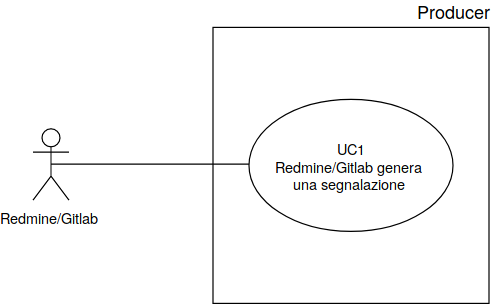
\includegraphics[width=0.7\textwidth]{img/UC1.png}\\
				\caption{UC\theuccount.2-GP -  Producer GitLab invia messaggio di issue al Gestore Personale}
			\end{figure}
			\begin{itemize}
				\item \textbf{Codice}: UC\theuccount.2-GP.
				\item \textbf{Titolo}:  Producer GitLab invia messaggio di issue al Gestore Personale.
				\item \textbf{Attori primari}: Producer GitLab.
				\item \textbf{Descrizione}: il Producer GitLab, dopo aver ricevuto una segnalazione di issue da GitLab,
				controlla se la issue è appena stata creata o si tratta di una modifica di
				una issue preesistente. Il messaggio elaborato, una volta elaborato, conterrà i campi:
				\begin{itemize}
					\item Project
					\item Topic
					\item Subject e opzionalmente:
					\begin{itemize}
						\item Description
						\item Due Date
						\item Milestone
						\item Assignee
					\end{itemize}
				\end{itemize}
				\item \textbf{Precondizione}: il Producer GitLab ha ricevuto una segnalazione da GitLab.
				\item \textbf{Postcondizione}: il Producer GitLab ha inviato al Gestore Personale il messaggio \newline elaborato.
				\item \textbf{Scenario principale}: 
				\begin{enumerate}
					\item Producer GitLab procede all'invio di un messaggio di
					issue al Gestore Personale.
				\end{enumerate}
				
			\end{itemize}
		
			\subparagraph{UC\theuccount.2.1-GP - Producer GitLab invia messaggio di una nuova issue al Gestore Personale}
				\begin{figure}[H]
					\centering
					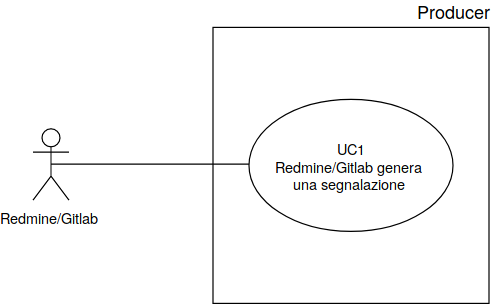
\includegraphics[width=0.7\textwidth]{img/UC1.png}\\
					\caption{UC\theuccount.2.1-GP - Producer GitLab invia messaggio di una nuova issue al Gestore Personale}
				\end{figure}
				\begin{itemize}
					\item \textbf{Codice}: UC\theuccount.2.1-GP.
					\item \textbf{Titolo}: Producer GitLab invia messaggio di una nuova issue al Gestore Personale.
					\item \textbf{Attori primari}: Producer GitLab.
					\item \textbf{Descrizione}: il Producer GitLab, dopo aver ricevuto una segnalazione di una nuova issue
					da GitLab, elabora il messaggio che conterrà i campi:
					\begin{itemize}
						\item Project
						\item Topic
						\item Subject e opzionalmente:
						\begin{itemize}
							\item Description
							\item Due Date
							\item Milestone
							\item Assignee
						\end{itemize}
					\end{itemize}
					\item \textbf{Precondizione}: il Producer GitLab ha ricevuto una segnalazione da GitLab.
					\item \textbf{Postcondizione}: il Producer GitLab ha inviato al Gestore Personale il messaggio elaborato di nuova issue.
					\item \textbf{Scenario principale}: 
					\begin{enumerate}
						\item Producer GitLab procede all'invio di un messaggio di
						nuova issue al Gestore Personale.
					\end{enumerate}
					
				\end{itemize}
		
			\subparagraph{UC\theuccount.2.2-GP - Producer GitLab invia messaggio di modifica di una issue al Gestore Personale}
				\begin{figure}[H]
					\centering
					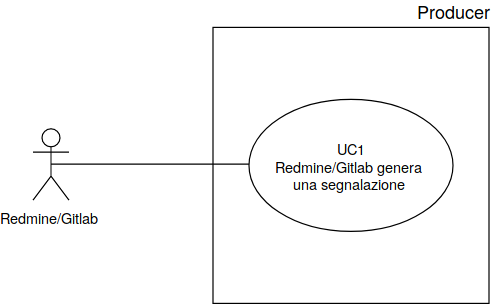
\includegraphics[width=0.7\textwidth]{img/UC1.png}\\
					\caption{UC\theuccount.2.2-GP - Producer GitLab invia messaggio di modifica di una issue al Gestore Personale}
				\end{figure}
				\begin{itemize}
					\item \textbf{Codice}: UC\theuccount.2.2-GP.
					\item \textbf{Titolo}: Producer GitLab invia messaggio di modifica di una issue al Gestore Personale.
					\item \textbf{Attori primari}: Producer GitLab.
					\item \textbf{Descrizione}: il Producer GitLab, dopo aver ricevuto una segnalazione di modifica di una issue da
					GitLab, controlla se sono stati modificati i campi Label o Title.
					In caso positivo, viene inviato un messaggio elaborato al Gestore Personale, il quale conterrà:
					\begin{itemize}
						\item Project
						\item Topic
						\item Subject e opzionalmente:
						\begin{itemize}
							\item Description
							\item Due Date
							\item Milestone
							\item Assignee
						\end{itemize}
					\end{itemize}
					\item \textbf{Precondizione}: il Producer GitLab ha ricevuto una segnalazione da GitLab.
					\item \textbf{Postcondizione}: il Producer GitLab ha inviato al Gestore Personale il messaggio elaborato di modifica issue.
					\item \textbf{Scenario principale}: 
					\begin{enumerate}
						\item Producer GitLab procede all'invio di un messaggio di modifica issue al Gestore Personale.
					\end{enumerate}
					\item \textbf{Estensioni}: 
					\begin{enumerate}
						\item Ci sono dei messaggi non validi e vengono scartati [UCGP\theuccount.2.3].
					\end{enumerate}
				\end{itemize}
		
			\subparagraph{UC\theuccount.2.3-GP - Producer GitLab scarta i messaggi non validi}
				\begin{figure}[H]
					\centering
					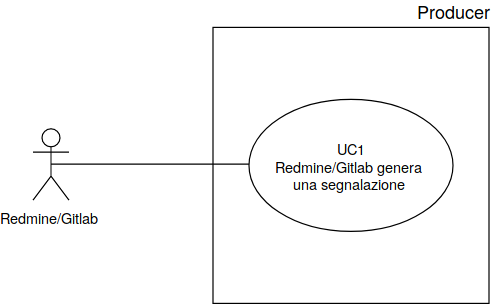
\includegraphics[width=0.7\textwidth]{img/UC1.png}\\
					\caption{UC\theuccount.2.3-GP - Producer GitLab scarta i messaggi non validi}
				\end{figure}
				\begin{itemize}
					\item \textbf{Codice}: UC\theuccount.2.3-GP.
					\item \textbf{Titolo}: Producer GitLab scarta i messaggi non validi.
					\item \textbf{Attori primari}: Producer GitLab.
					\item \textbf{Descrizione}: il Producer GitLab, dopo aver ricevuto una segnalazione di una modifica issue da GitLab, controlla
					se sono state modificati i campi Label o Title. In caso negativo, il messaggio viene scartato.
					\item \textbf{Precondizione}: il Producer GitLab ha ricevuto una segnalazione da GitLab.
					\item \textbf{Postcondizione}: il Producer GitLab ha scartato il messaggio.
					\item \textbf{Scenario principale}: 
					\begin{enumerate}
						\item Producer GitLab scarta i messaggi non validi.
					\end{enumerate}
				\end{itemize}

\stepcounter{uccount}

\subsubsection{UC\theuccount-CT - Gestore Personale invia il messaggio finale al Consumer Telegram}
	\begin{figure}[H]
		\centering
		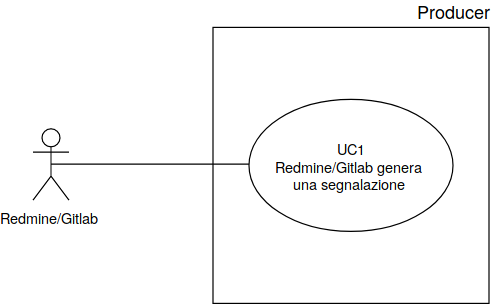
\includegraphics[width=0.7\textwidth]{img/UC1.png}\\
		\caption{UC\theuccount-CT - Gestore Personale invia il messaggio finale al Consumer Telegram}
	\end{figure}
	\begin{itemize}
		\item \textbf{Codice}: UC\theuccount-CT.
		\item \textbf{Titolo}: Gestore Personale invia il messaggio finale al Consumer Telegram.
		\item \textbf{Attori primari}: Gestore Personale.
		\item \textbf{Descrizione}: il Gestore Personale, dopo aver ricevuto il messaggio elaborato dai Producer Redmine o GitLab,
		valuta il campo Topic del messaggio, controlla chi è iscritto a quel Topic, se la persona è disponibile, e se vuole ricevere
		il messaggio tramite Telegram. Se tutte queste condizioni sono verificate, viene preparato il messaggio finale da inviare
		all'utente e inviato al Consumer Telegram. Il messaggio finale, una volta elaborato, conterrà i campi:
		\begin{itemize}
			\item Id della chat del destinatario
			\item Applicazione di provenienza
			\item Ora di invio
			\item Tipo di segnalazione(commit, issue)
			\item Project
			\item Topic
			\item Subject e opzionalmente
		 	\begin{itemize}
				\item Description
				\item Due date
				\item Milestone
				\item Assignee
			\end{itemize}
		\end{itemize}
		\item \textbf{Precondizione}: il Gestore Personale ha ricevuto il messaggio elaborato dai Producer Redmine o GitLab.
		\item \textbf{Postcondizione}: Il Gestore Personale ha inviato il messaggio finale al Consumer Telegram.
		\item \textbf{Scenario principale}: 
		\begin{enumerate}
			\item Gestore Personale procede all'invio del messaggio finale al Consumer Telegram.
		\end{enumerate}
		
	\end{itemize}

\stepcounter{uccount}

\subsubsection{UC\theuccount-CE - Gestore Personale invia il messaggio finale al Consumer Email}
	\begin{figure}[H]
		\centering
		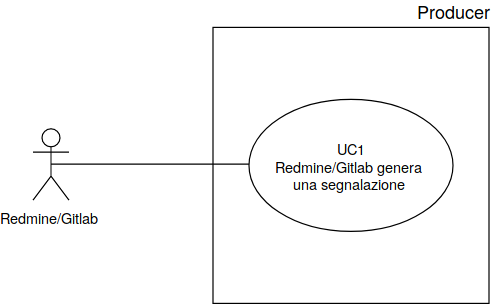
\includegraphics[width=0.7\textwidth]{img/UC1.png}\\
		\caption{UC\theuccount-CE - Gestore Personale invia il messaggio finale al Consumer Email}
	\end{figure}
	\begin{itemize}
		\item \textbf{Codice}: UC\theuccount-CE.
		\item \textbf{Titolo}: Gestore Personale invia il messaggio finale al Consumer Email.
		\item \textbf{Attori primari}: Gestore Personale.
		\item \textbf{Descrizione}: il Gestore Personale, dopo aver ricevuto il messaggio elaborato dai Producer Redmine o GitLab,
		valuta il campo Topic del messaggio, controlla chi è iscritto a quel Topic, se la persona è disponibile, e se vuole ricevere
		il messaggio tramite email. Se tutte queste condizioni sono verificate, viene preparato il messaggio finale da inviare al
		Consumer Email. Il messaggio finale, una volta elaborato, conterrà i campi:
		\begin{itemize}
			\item Email del destinatario
			\item Applicazione di provenienza
			\item Ora di invio
			\item Tipo di segnalazione(commit, issue)
			\item Project
			\item Topic
			\item Subject e opzionalmente
		 	\begin{itemize}
				\item Description
				\item Due date
				\item Milestone
				\item Assignee
			\end{itemize}
		\end{itemize}
		\item \textbf{Precondizione}: il Gestore Personale ha ricevuto il messaggio elaborato dai Producer Redmine o GitLab.
		\item \textbf{Postcondizione}: Il Gestore Personale ha inviato il messaggio finale al Consumer Email.
		\item \textbf{Scenario principale}: 
		\begin{enumerate}
			\item Gestore Personale procede all'invio del messaggio finale al Consumer Email.
		\end{enumerate}
		
	\end{itemize}

\stepcounter{uccount}

\subsubsection{UC\theuccount-BT - Consumer Telegram inoltra il messaggio finale al bot Telegram}
	\begin{figure}[H]
		\centering
		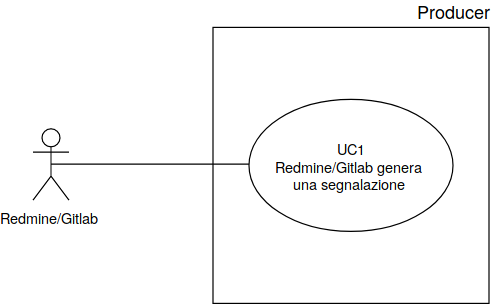
\includegraphics[width=0.7\textwidth]{img/UC1.png}\\
		\caption{UC\theuccount-BT - Consumer Telegram inoltra il messaggio finale al bot Telegram}
	\end{figure}
	\begin{itemize}
		\item \textbf{Codice}: UC\theuccount-BT.
		\item \textbf{Titolo}: Consumer Telegram inoltra il messaggio finale al bot Telegram.
		\item \textbf{Attori primari}: Consumer Telegram.
		\item \textbf{Descrizione}: il Consumer Telegram inoltra il messaggio finale al bot Telegram, il quale notifica il destinatario finale attraverso Telegram.
		\item \textbf{Precondizione}: il Consumer Telegram ha ricevuto almeno un messaggio.
		\item \textbf{Postcondizione}: il bot Telegram ha ricevuto il messaggio finale con successo.
		\item \textbf{Scenario principale}: 
		\begin{enumerate}
			\item Consumer Telegram procede all'inoltro del messaggio finale al bot Telegram.
		\end{enumerate}
		
	\end{itemize}

\stepcounter{uccount}

\subsubsection{UC\theuccount-SE - Consumer Email inoltra il messaggio finale al server Email}
	\begin{figure}[H]
		\centering
		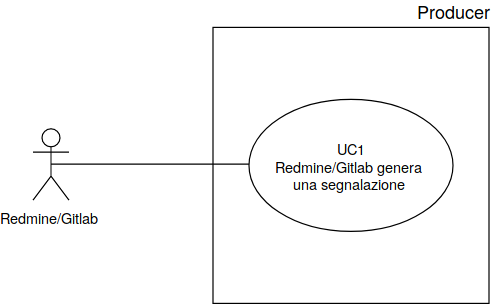
\includegraphics[width=0.7\textwidth]{img/UC1.png}\\
		\caption{UC\theuccount-SE - Consumer Email inoltra il messaggio finale al server Email}
	\end{figure}
	\begin{itemize}
		\item \textbf{Codice}: UC\theuccount-SE.
		\item \textbf{Titolo}: Consumer Email inoltra il messaggio finale al server Email.
		\item \textbf{Attori primari}: Consumer Email.
		\item \textbf{Descrizione}: il Consumer Email inoltra il messaggio finale al server Email, il quale notifica il destinatario finale attraverso una Email.
		\item \textbf{Precondizione}: il Consumer Email ha ricevuto almeno un messaggio.
		\item \textbf{Postcondizione}: il server Email ha ricevuto il messaggio finale con successo.
		\item \textbf{Scenario principale}: 
		\begin{enumerate}
			\item Consumer Email procede all'inoltro del messaggio finale al server Email.
		\end{enumerate}
		
	\end{itemize}

\stepcounter{uccount}

\subsubsection{UC\theuccount-GP - Accesso}
		\begin{figure}[H]
			\centering
				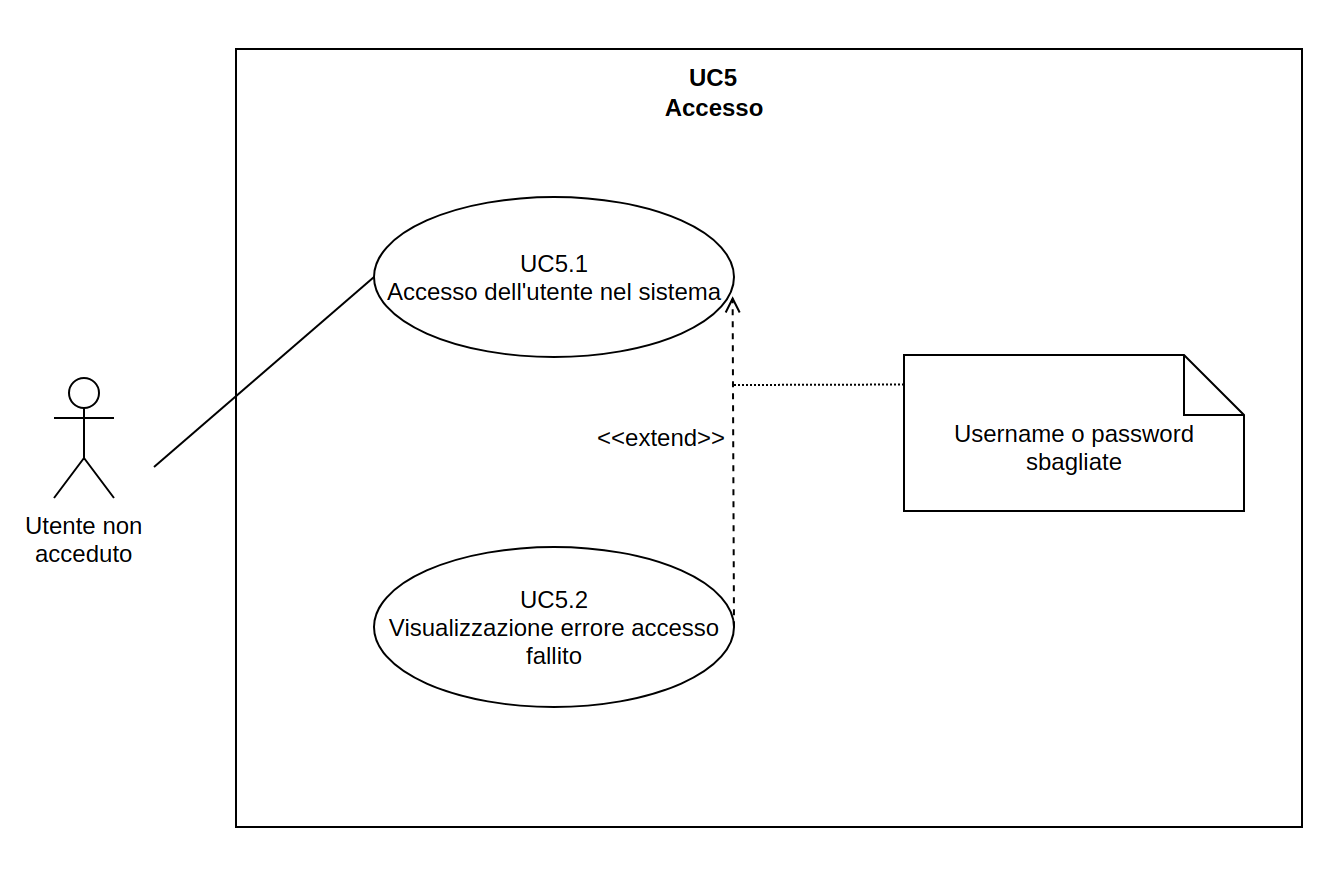
\includegraphics[width=\columnwidth]{img/UC5.png}\\
			\caption{UC\theuccount-GP - Accesso}
		\end{figure}
	\begin{itemize}
		\item \textbf{Codice}: UC\theuccount-GP.
		\item \textbf{Titolo}: accesso.
		\item \textbf{Attori primari}: utente non acceduto.
		\item \textbf{Descrizione}: l'utente richiede di accedere al sistema attraverso un form dove inserisce l'username.
		\item \textbf{Precondizione}: il sistema considera l’utilizzatore di esso come un utente non acceduto.
		\item \textbf{Postcondizione}: il sistema riconosce l'utilizzatore di esso come utente acceduto.
		\item \textbf{Scenario Principale}:
		\begin{enumerate}
			\item L'utente non ancora riconosciuto dal sistema effettua l'accesso inserendo il proprio username.
		\end{enumerate}
	\end{itemize}
	
	\paragraph{UC\theuccount.1-GP - Accesso dell'utente nel sistema}
		\begin{figure}[H]
			\centering
				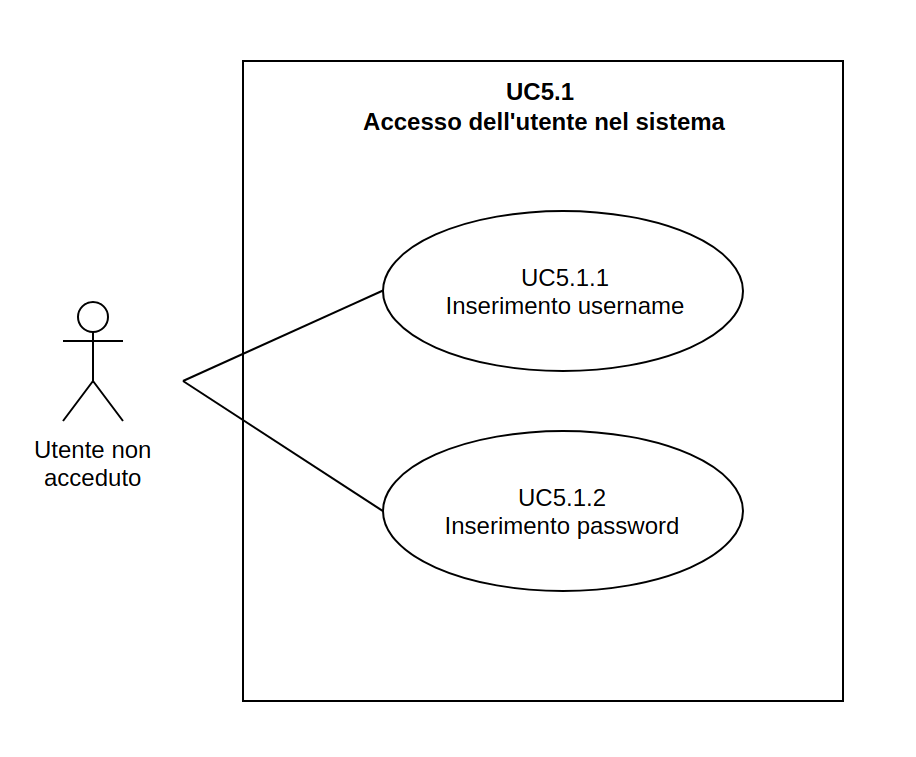
\includegraphics[width=\columnwidth]{img/UC5_1.png}\\
			\caption{UC\theuccount.1-GP - Accesso dell'utente nel sistema}
		\end{figure}
		\begin{itemize}
			\item \textbf{Codice}: UC\theuccount.1-GP.
			\item \textbf{Titolo}: accesso dell'utente nel sistema.
			\item \textbf{Attori primari}: utente non acceduto.
			\item \textbf{Descrizione}: l'utente attende l'accesso al sistema.
			\item \textbf{Precondizione}: il sistema riconosce l'utilizzatore come un utente non acceduto.
			\item \textbf{Postcondizione}: il sistema riconosce l'utente con successo.
			\item \textbf{Scenario Principale}:
			\begin{enumerate}
				\item L’utente non ancora riconosciuto dal sistema richiede l'accesso attraverso l'inserimento dell'username.
			\end{enumerate}
			\item \textbf{Estensioni}:
			\begin{enumerate}
				\item L'accesso non va a buon fine e viene visualizzato un errore avvisando l'utente [UC5.2].
			\end{enumerate}
		\end{itemize}

		\subparagraph{UC\theuccount.1.1-GP - Inserimento username}
			\begin{itemize}
				\item \textbf{Codice}: UC\theuccount.1.1-GP.
				\item \textbf{Titolo}: inserimento username.
				\item \textbf{Attori primari}: utente non acceduto.
				\item \textbf{Descrizione}: l'utente inserisce l'username.
				\item \textbf{Precondizione}: il sistema offre l'interfaccia grafica adatta all'inserimento dell'username.
				\item \textbf{Postcondizione}: l'utente ha inserito l'username desiderato.
				\item \textbf{Scenario Principale}:
				\begin{enumerate}
					\item L'utente inserisce l'username per autenticarsi.
				\end{enumerate}
			\end{itemize}

	\paragraph{UC\theuccount.2-GP - Errore username inesistente}
		\begin{itemize}
			\item \textbf{Codice}: UC\theuccount.1.2-GP.
			\item \textbf{Titolo}: errore username inesistente.
			\item \textbf{Attori primari}: utente non acceduto.
			\item \textbf{Descrizione}: l'utente viene avvisato che ha inserito un username errato.
			\item \textbf{Precondizione}: il sistema riceve una richiesta di accesso da parte di un utente che
			fornisce uno username errato. 
			\item \textbf{Postcondizione}: il sistema comunica all'utilizzatore l'errore.
			\item \textbf{Scenario Principale}:
			\begin{enumerate}
				\item L'utente visualizza il messaggio d'errore.
			\end{enumerate}
		\end{itemize}


\stepcounter{uccount}

\subsubsection{UC\theuccount-GP - Uscita dell'utente dal sistema}
		\begin{figure}[H]
			\centering
				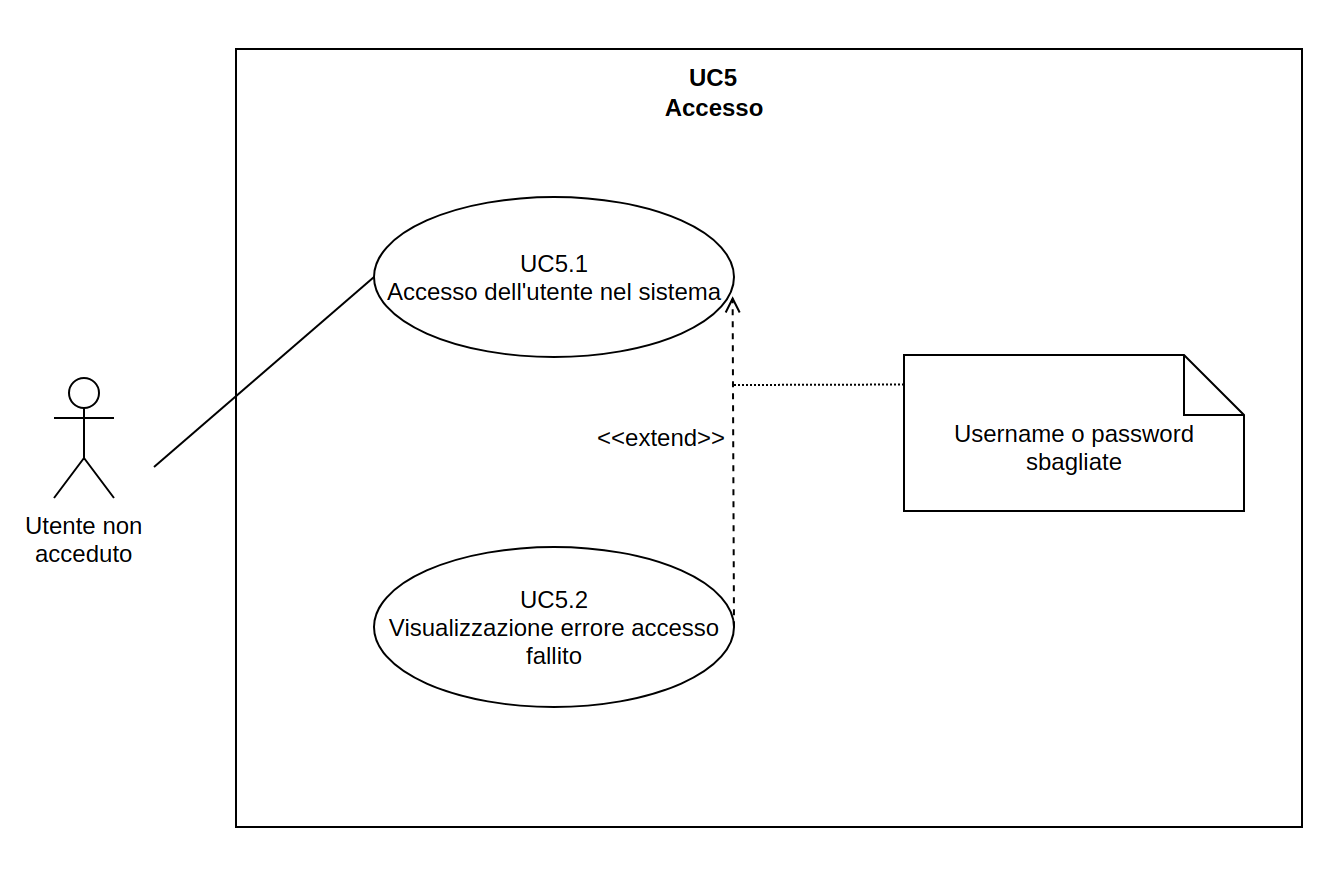
\includegraphics[width=\columnwidth]{img/UC5.png}\\
			\caption{UC\theuccount-GP - Accesso}
		\end{figure}
	\begin{itemize}
		\item \textbf{Codice}: UC\theuccount-GP.
		\item \textbf{Titolo}: uscita dell'utente dal sistema.
		\item \textbf{Attori primari}: utente acceduto.
		\item \textbf{Descrizione}: l'utente esce dal sistema ed ha la possibilità di rientrarci come
		un diverso utente o come lo stesso di prima.
		\item \textbf{Precondizione}: l'utente è all'interno del sistema.
		\item \textbf{Postcondizione}: l'utente si trova a poter accedere nuovamente nel sistema.
		\item \textbf{Scenario Principale}:
		\begin{enumerate}
			\item L'utente riconosciuto dal sistema effettua l'uscita.
		\end{enumerate}
	\end{itemize}

\stepcounter{uccount}

\subsubsection{UC\theuccount-GP - Aggiunta nuovo utente}
		\begin{figure}[H]
			\centering
				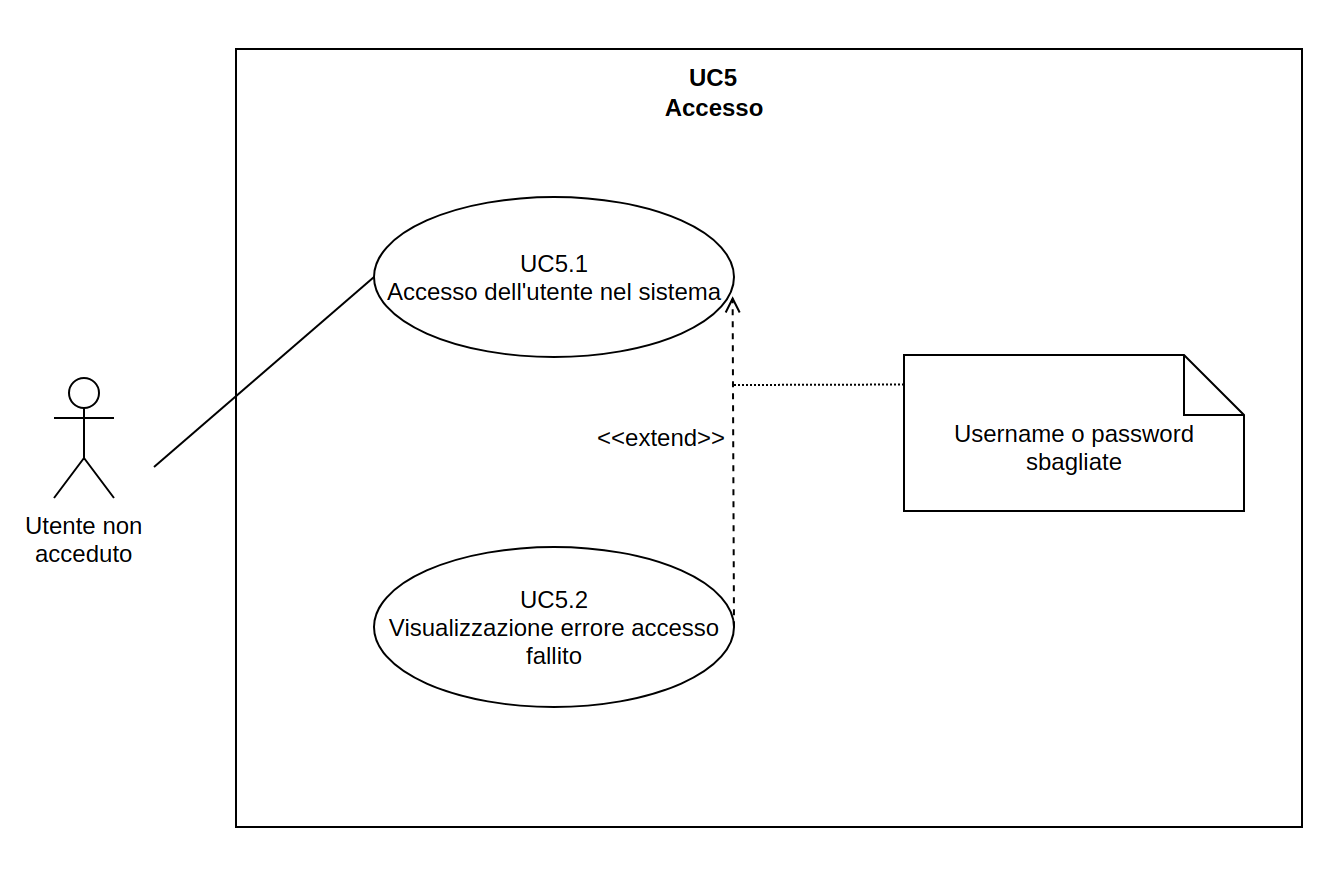
\includegraphics[width=\columnwidth]{img/UC5.png}\\
			\caption{UC\theuccount-GP - Aggiunta nuovo utente}
		\end{figure}
	\begin{itemize}
		\item \textbf{Codice}: UC\theuccount-GP.
		\item \textbf{Titolo}: aggiunta nuovo utente.
		\item \textbf{Attori primari}: utente acceduto.
		\item \textbf{Descrizione}: l'utente aggiunge un nuovo utente nel sistema.
		\item \textbf{Precondizione}: un nuovo utente deve essere aggiunto nel sistema.
		\item \textbf{Postcondizione}: un utente viene aggiunto al sistema.
		\item \textbf{Scenario Principale}:
		\begin{enumerate}
			\item Utente acceduto procede all'aggiunta di un nuovo utente.
		\end{enumerate}
	\end{itemize}

	\paragraph{UC\theuccount.1-GP - Utente aggiunto con successo}
		\begin{figure}[H]
			\centering
			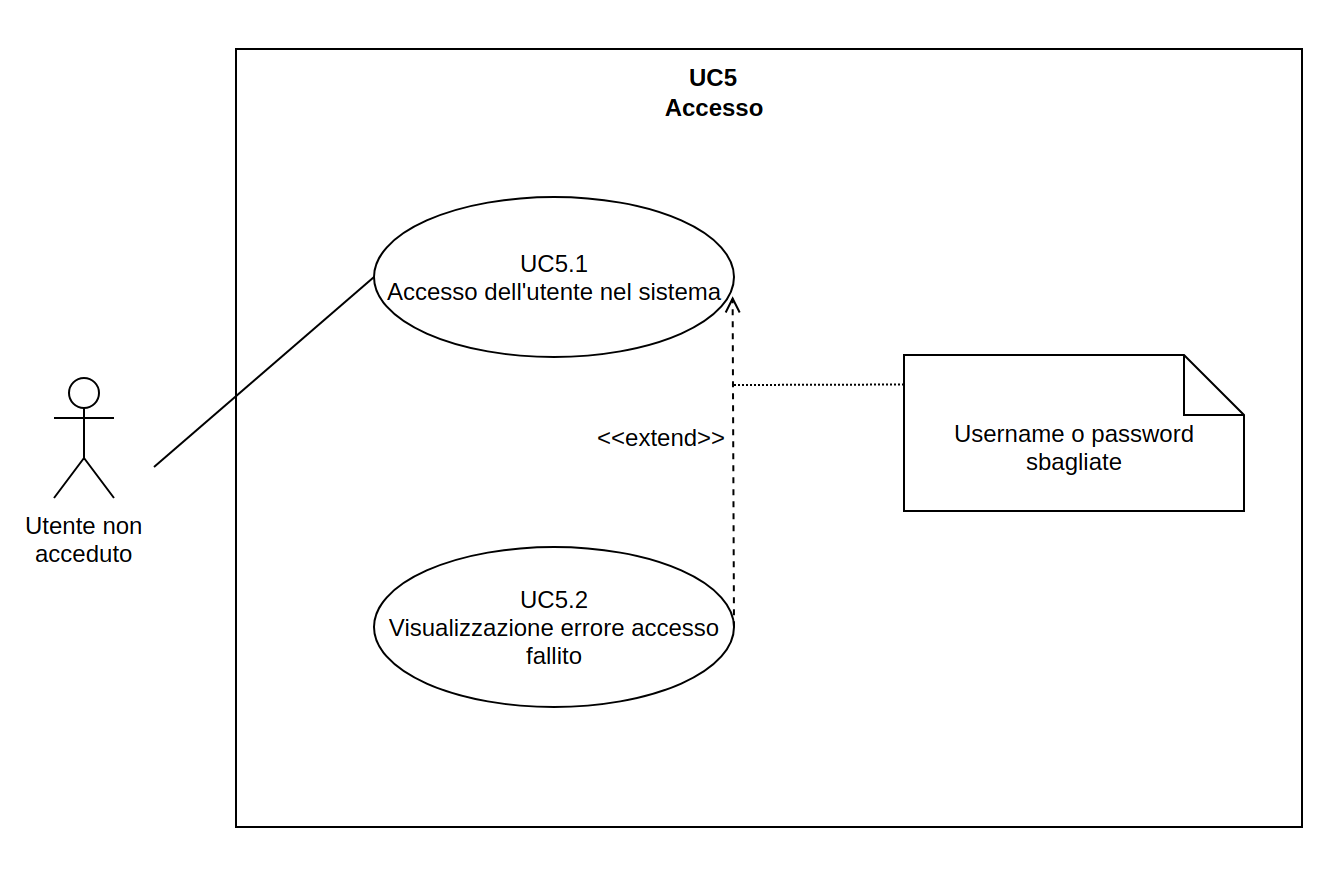
\includegraphics[width=\columnwidth]{img/UC5.png}\\
			\caption{UC\theuccount.1-GP - Utente aggiunto con successo}
		\end{figure}
		\begin{itemize}
			\item \textbf{Codice}: UC\theuccount.1-GP.
			\item \textbf{Titolo}: utente aggiunto con successo.
			\item \textbf{Attori primari}: utente acceduto.
			\item \textbf{Descrizione}: un nuovo utente viene inserito con successo nel sistema.
			\item \textbf{Precondizione}: un nuovo utente deve essere aggiunto nel sistema.
			\item \textbf{Postcondizione}: un utente viene aggiunto al sistema.
			\item \textbf{Scenario Principale}:
			\begin{enumerate}
				\item Utente acceduto procede all'aggiunta di un nuovo utente.
			\end{enumerate}
			\item \textbf{Estensioni}:
			\begin{itemize}
				\item Errore utente già presente nel sistema[UC13-GP].
			\end{itemize}
		\end{itemize}

		\subparagraph{UC\theuccount.1.1-GP - Inserimento nome utente}
			\begin{figure}[H]
				\centering
				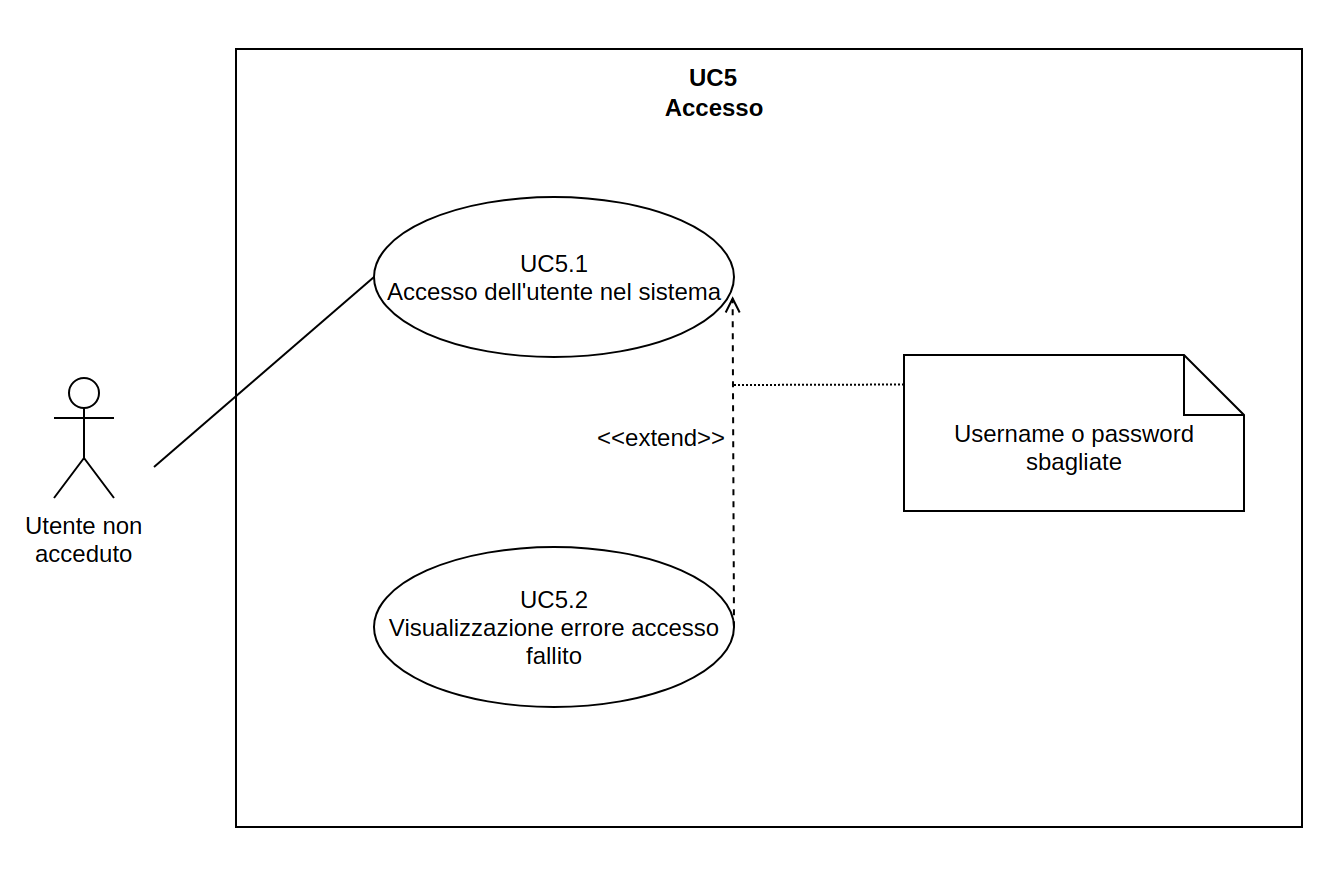
\includegraphics[width=\columnwidth]{img/UC5.png}\\
				\caption{UC\theuccount.1.1-GP - Inserimento nome utente}
			\end{figure}
			\begin{itemize}
				\item \textbf{Codice}: UC\theuccount.1.1-GP.
				\item \textbf{Titolo}: inserimento nome utente.
				\item \textbf{Attori primari}: utente acceduto.
				\item \textbf{Descrizione}: l'utente inserisce il nominativo dell'utente appena aggiunto.
				\item \textbf{Precondizione}: un nuovo utente deve essere aggiunto nel sistema.
				\item \textbf{Postcondizione}: il nome è stato aggiunto.
				\item \textbf{Scenario Principale}:
				\begin{enumerate}
					\item Utente acceduto procede all'aggiunta del nominativo del nuovo utente.
				\end{enumerate}
			\end{itemize}

			\subparagraph{UC\theuccount.1.2-GP - Inserimento cognome utente}
				\begin{figure}[H]
					\centering
					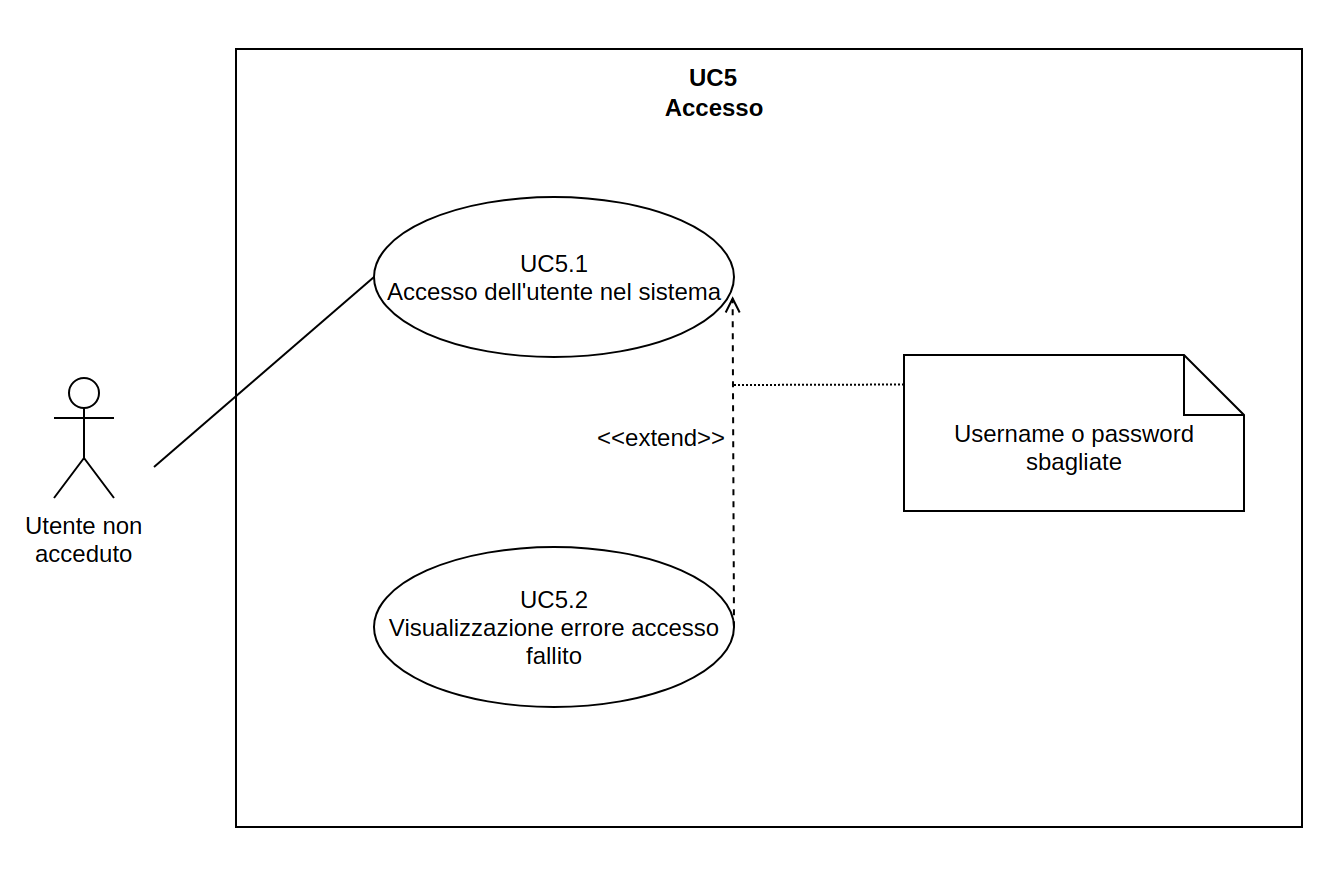
\includegraphics[width=\columnwidth]{img/UC5.png}\\
					\caption{UC\theuccount.1.2-GP - Inserimento cognome utente}
				\end{figure}
				\begin{itemize}
					\item \textbf{Codice}: UC\theuccount.1.2-GP.
					\item \textbf{Titolo}: inserimento cognome utente.
					\item \textbf{Attori primari}: utente acceduto.
					\item \textbf{Descrizione}: l'utente inserisce il cognome dell'utente appena aggiunto.
					\item \textbf{Precondizione}: un nuovo utente deve essere aggiunto nel sistema.
					\item \textbf{Postcondizione}: il cognome è stato aggiunto.
					\item \textbf{Scenario Principale}:
					\begin{enumerate}
						\item Utente acceduto procede all'aggiunta del cognome del nuovo utente.
					\end{enumerate}
				\end{itemize}

				\subparagraph{UC\theuccount.1.3-GP - Inserimento contatto Email}
					\begin{figure}[H]
						\centering
						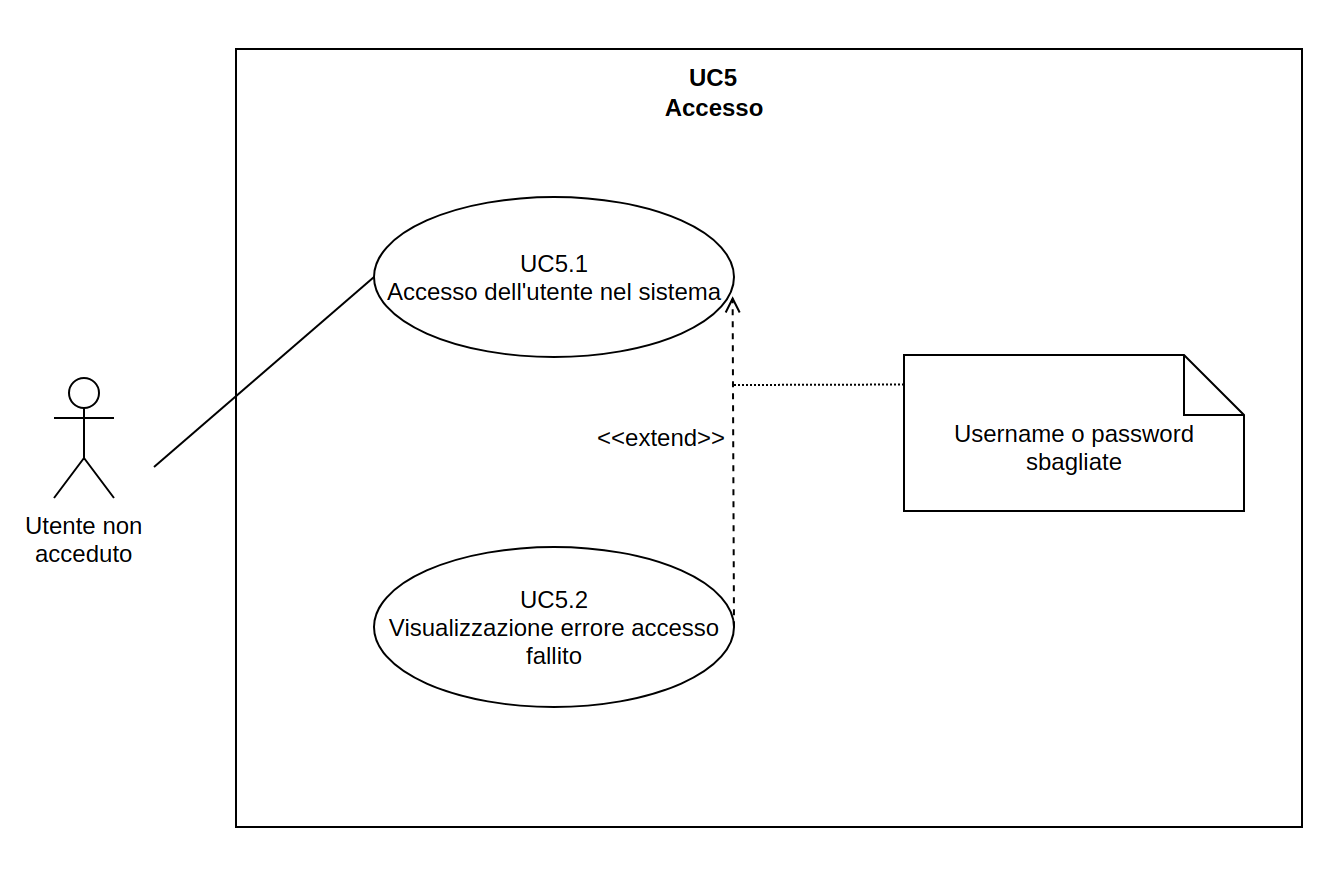
\includegraphics[width=\columnwidth]{img/UC5.png}\\
						\caption{UC\theuccount.1.3-GP - Inserimento contatto Email}
					\end{figure}
					\begin{itemize}
						\item \textbf{Codice}: UC\theuccount.1.3-GP.
						\item \textbf{Titolo}: inserimento contatto Email.
						\item \textbf{Attori primari}: utente acceduto.
						\item \textbf{Descrizione}: l'utente inserisce il contatto Email dell'utente appena aggiunto.
						\item \textbf{Precondizione}: un nuovo utente deve essere aggiunto nel sistema.
						\item \textbf{Postcondizione}: il contatto Email è stato aggiunto.
						\item \textbf{Scenario Principale}:
						\begin{enumerate}
							\item Utente acceduto procede all'aggiunta del contatto Email del nuovo utente.
						\end{enumerate}
				\end{itemize}

				\subparagraph{UC\theuccount.1.4-GP - Inserimento contatto Telegram}
					\begin{figure}[H]
						\centering
						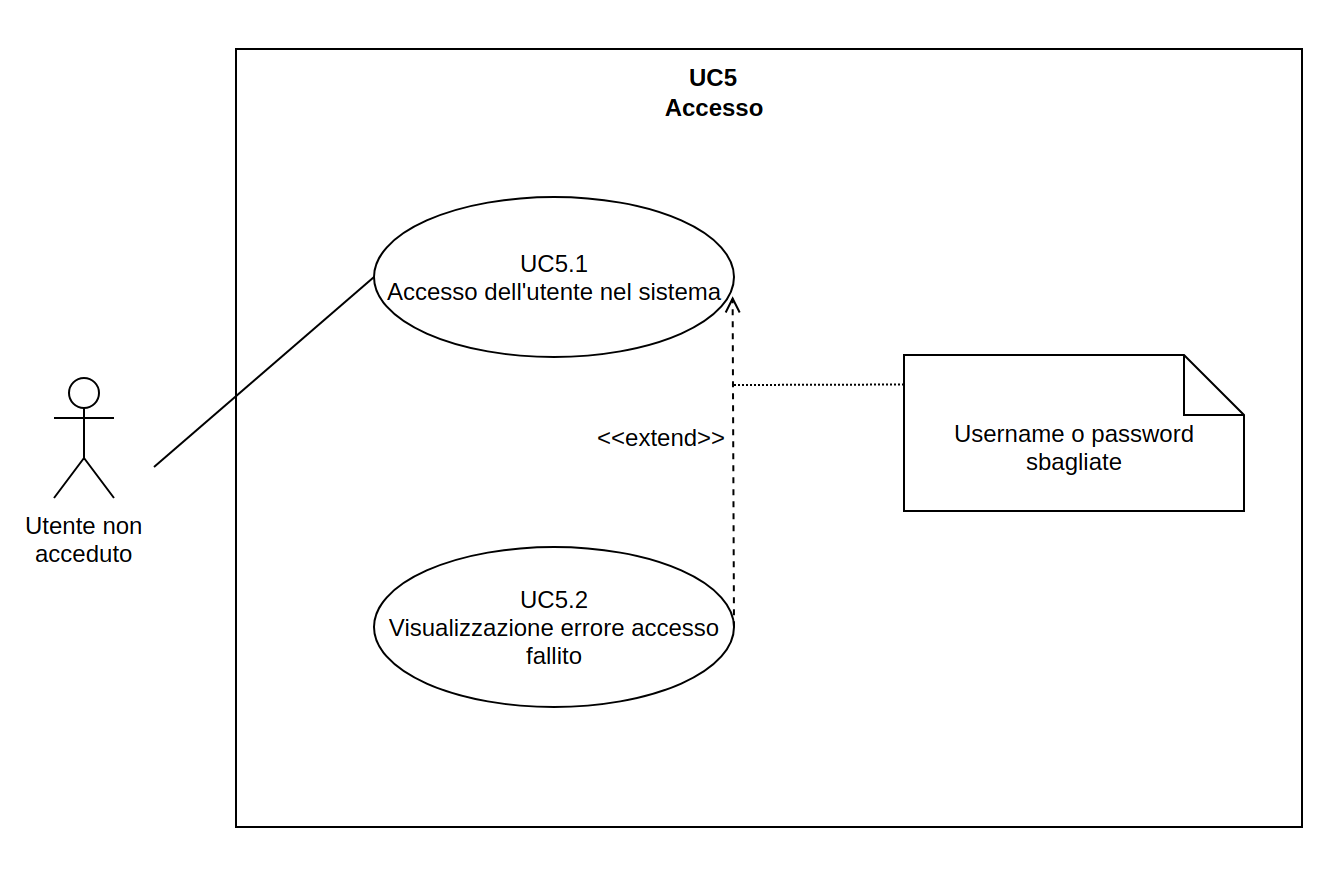
\includegraphics[width=\columnwidth]{img/UC5.png}\\
						\caption{UC\theuccount.1.4-GP - Inserimento contatto Telegram}
					\end{figure}
					\begin{itemize}
						\item \textbf{Codice}: UC\theuccount.1.4-GP.
						\item \textbf{Titolo}: inserimento contatto Telegram.
						\item \textbf{Attori primari}: utente acceduto.
						\item \textbf{Descrizione}: l'utente inserisce il contatto Telegram dell'utente appena aggiunto.
						\item \textbf{Precondizione}: un nuovo utente deve essere aggiunto nel sistema.
						\item \textbf{Postcondizione}: il contatto Telegram è stato aggiunto.
						\item \textbf{Scenario Principale}:
						\begin{enumerate}
							\item Utente acceduto procede all'aggiunta del contatto Telegram del nuovo utente.
						\end{enumerate}
					\end{itemize}

			\paragraph{UC\theuccount.2-GP - Errore utente già presente nel sistema}
				\begin{figure}[H]
					\centering
					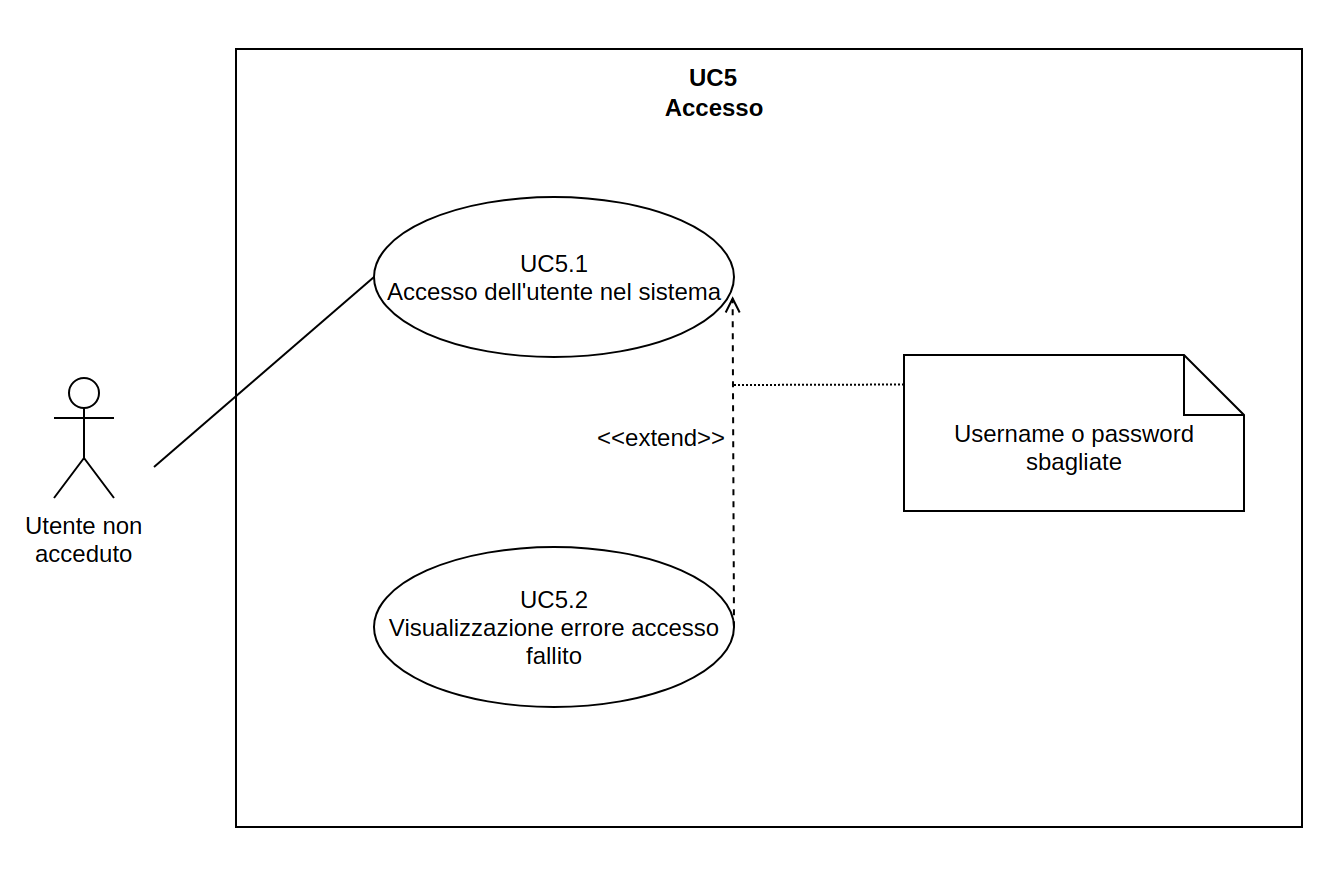
\includegraphics[width=\columnwidth]{img/UC5.png}\\
					\caption{UC\theuccount.2-GP - Errore utente già presente nel sistema}
				\end{figure}
				\begin{itemize}
					\item \textbf{Codice}: UC\theuccount.2-GP.
					\item \textbf{Titolo}: errore utente già presente nel sistema.
					\item \textbf{Attori primari}: utente acceduto.
					\item \textbf{Descrizione}: l’utente viene avvisato che i contatti Telegram o email immessi non sono univoci.
					\item \textbf{Precondizione}: un nuovo utente deve essere aggiunto nel sistema.
					\item \textbf{Postcondizione}: il sistema comunica all’utilizzatore l’errore e l'utente non viene inserito.
					\item \textbf{Scenario Principale}:
					\begin{enumerate}
						\item Utente acceduto visualizza il messaggio d'errore.
					\end{enumerate}
				\end{itemize}

\stepcounter{uccount}

\subsubsection{UC\theuccount-GP - Rimozione utente dal sistema}
		\begin{figure}[H]
			\centering
				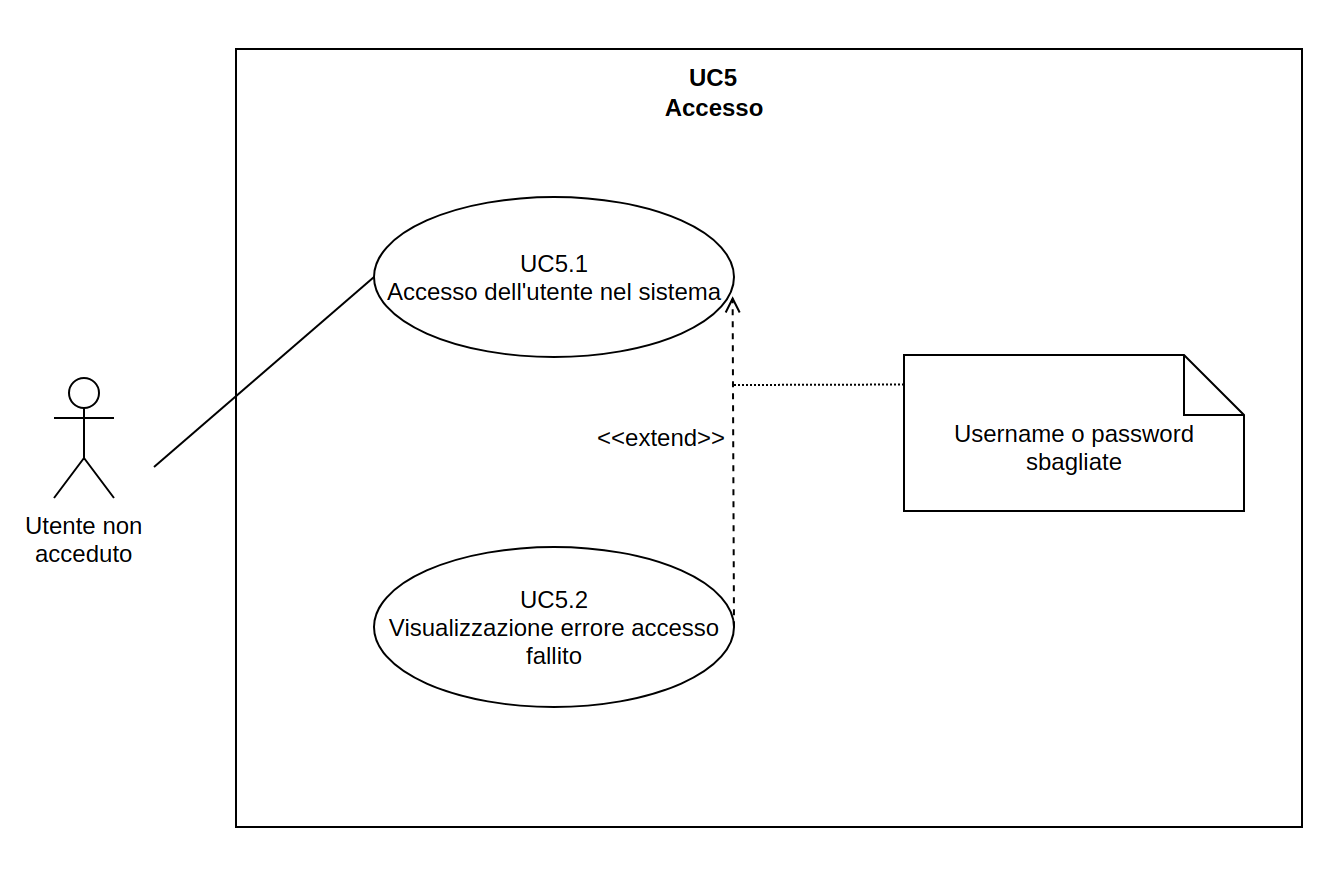
\includegraphics[width=\columnwidth]{img/UC5.png}\\
			\caption{UC\theuccount-GP - Rimozione utente dal sistema}
		\end{figure}
	\begin{itemize}
		\item \textbf{Codice}: UC\theuccount-GP.
		\item \textbf{Titolo}: Rimozione utente dal sistema.
		\item \textbf{Attori primari}: utente acceduto.
		\item \textbf{Descrizione}: l'utente rimuove l'utente desiderato dal sistema.
		\item \textbf{Precondizione}: un utente già presente deve essere rimosso dal sistema.
		\item \textbf{Postcondizione}: un utente viene rimosso dal sistema.
		\item \textbf{Scenario Principale}:
		\begin{enumerate}
			\item Utente acceduto procede alla rimozione di un utente.
		\end{enumerate}
\end{itemize}

	\paragraph{UC\theuccount.1-GP - Rimozione avvenuta con successo}
		\begin{figure}[H]
			\centering
			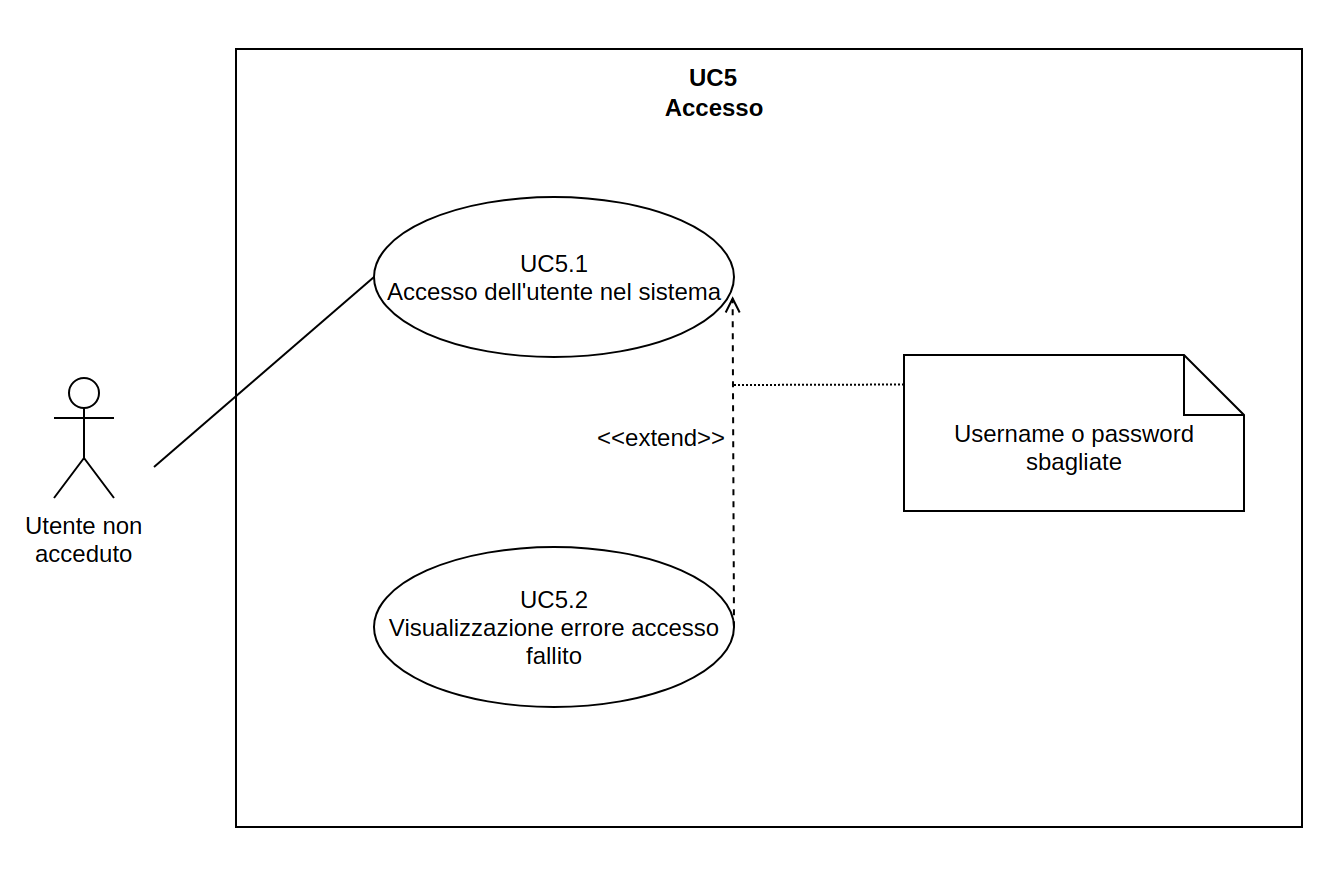
\includegraphics[width=\columnwidth]{img/UC5.png}\\
			\caption{UC\theuccount.1-GP - Rimozione avvenuta con successo}
		\end{figure}
		\begin{itemize}
			\item \textbf{Codice}: UC\theuccount.1-GP.
			\item \textbf{Titolo}: rimozione avvenuta con successo.
			\item \textbf{Attori primari}: utente acceduto.
			\item \textbf{Descrizione}: il contatto Email o Telegram desiderato è presente nel sistema,
			per cui la rimozione avviene con successo.
			\item \textbf{Precondizione}: un utente già presente deve essere rimosso dal sistema.
			\item \textbf{Postcondizione}: un utente con il contatto Email o Telegram inserito viene rimosso dal sistema.
			\item \textbf{Scenario Principale}:
			\begin{enumerate}
				\item Un utente viene rimosso.
			\end{enumerate}
			\item \textbf{Estensioni}:
			\begin{itemize}
				\item Errore contatto non presente nel sistema[UC14.2-GP].
			\end{itemize}
		\end{itemize}

			\subparagraph{UC\theuccount.1.1-GP - Inserimento contatto Email}
				\begin{figure}[H]
					\centering
					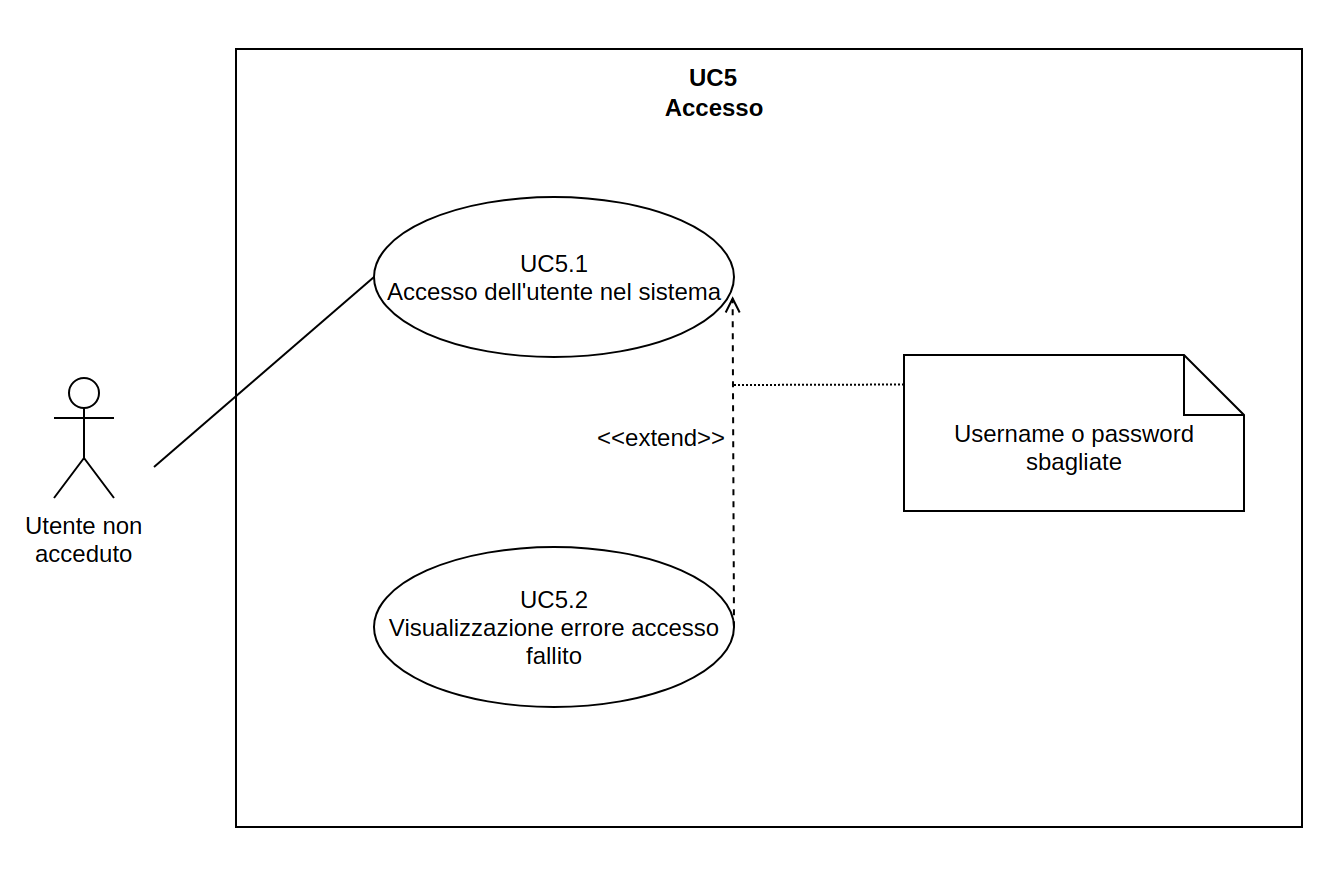
\includegraphics[width=\columnwidth]{img/UC5.png}\\
					\caption{UC\theuccount.1.1-GP - Inserimento contatto Email}
				\end{figure}
				\begin{itemize}
					\item \textbf{Codice}: UC\theuccount.1.1-GP.
					\item \textbf{Titolo}: inserimento contatto Email.
					\item \textbf{Attori primari}: utente acceduto.
					\item \textbf{Descrizione}: l'utente ha aggiunto il contatto Email relativo all'utente che vuole rimuovere.
					\item \textbf{Precondizione}: un utente già presente deve essere rimosso dal sistema.
					\item \textbf{Postcondizione}: il contatto Email è stato inserito.
					\item \textbf{Scenario Principale}:
					\begin{enumerate}
						\item Utente acceduto procede all'inserimento del contatto Email del utente da rimuovere.
					\end{enumerate}
				\end{itemize}

				\subparagraph{UC\theuccount.1.2-GP - Inserimento contatto Telegram}
					\begin{figure}[H]
						\centering
						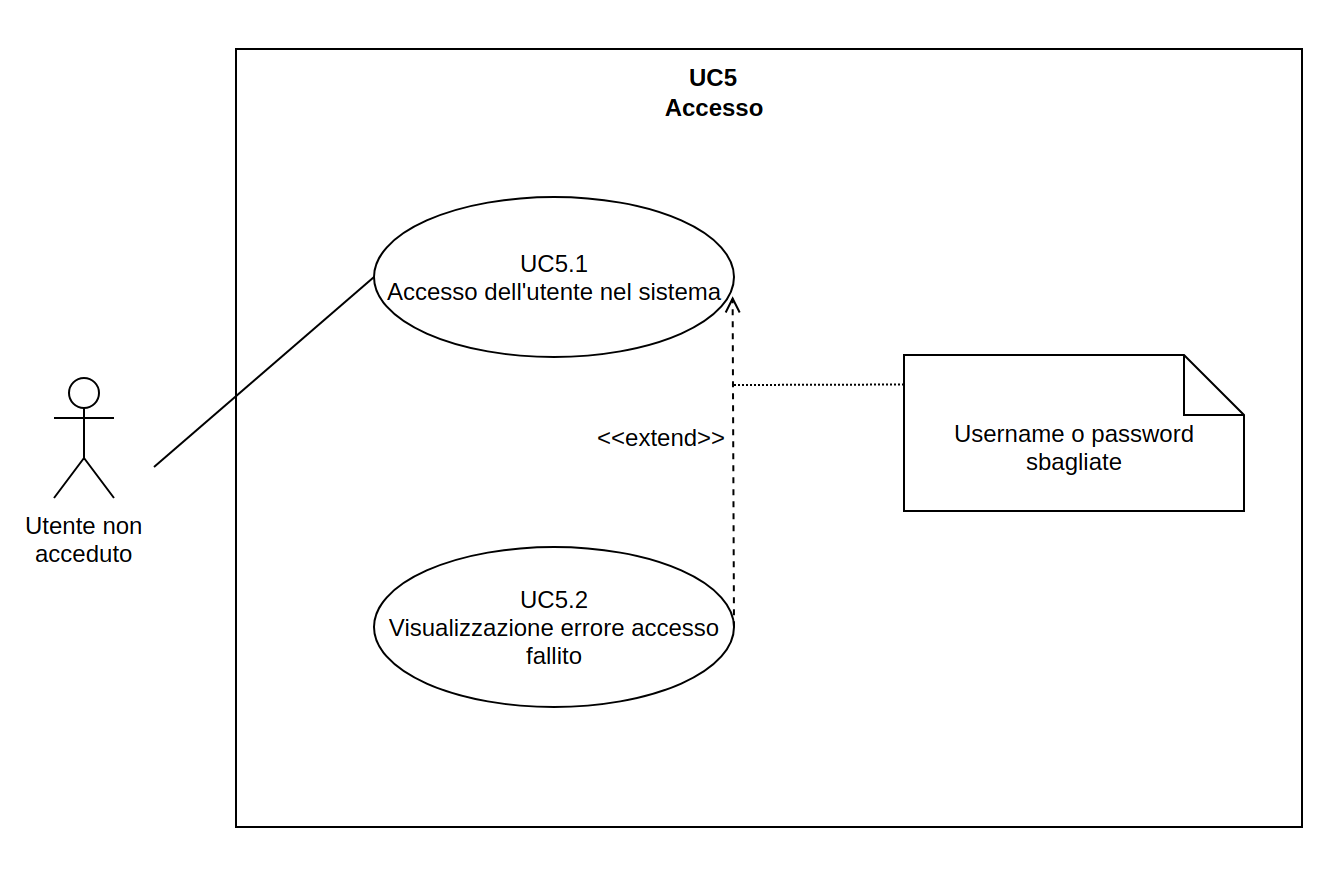
\includegraphics[width=\columnwidth]{img/UC5.png}\\
						\caption{UC\theuccount.1.2-GP - Inserimento contatto Telegram}
					\end{figure}
					\begin{itemize}
						\item \textbf{Codice}: UC\theuccount.1.2-GP.
						\item \textbf{Titolo}: inserimento contatto Telegram.
						\item \textbf{Attori primari}: utente acceduto.
						\item \textbf{Descrizione}: l'utente ha aggiunto il contatto Telegram relativo all'utente che vuole rimuovere.
						\item \textbf{Precondizione}: un utente già presente deve essere rimosso dal sistema.
						\item \textbf{Postcondizione}: il contatto Telegram è stato inserito.
						\item \textbf{Scenario Principale}:
						\begin{enumerate}
							\item Utente acceduto procede all'inserimento del contatto Telegram del utente da rimuovere.
						\end{enumerate}
					\end{itemize}

				\paragraph{UC\theuccount.2-GP - Errore contatto non presente nel sistema}
						\begin{figure}[H]
							\centering
							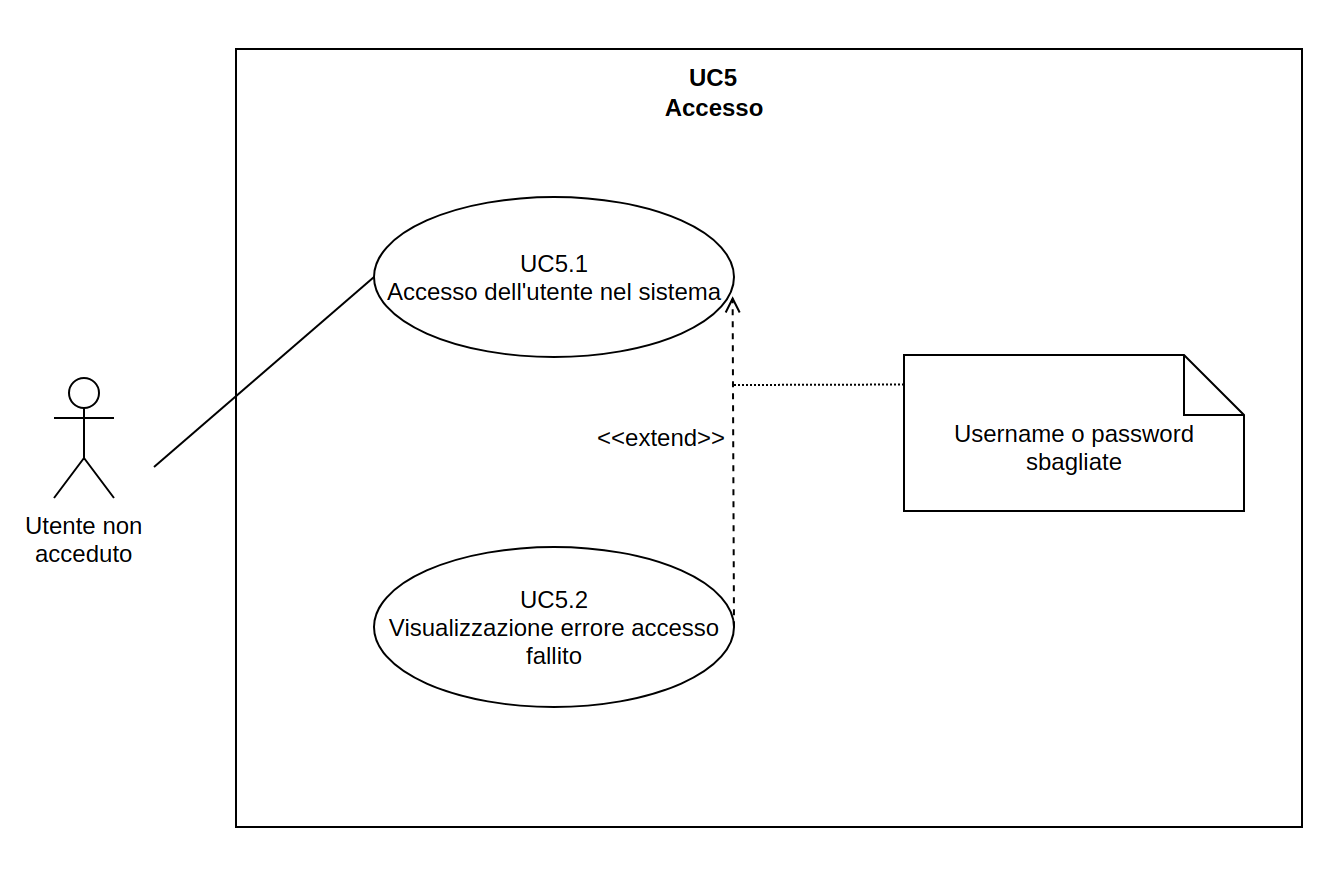
\includegraphics[width=\columnwidth]{img/UC5.png}\\
							\caption{UC\theuccount.2-GP - Errore contatto non presente nel sistema}
						\end{figure}
						\begin{itemize}
							\item \textbf{Codice}: UC\theuccount.2-GP.
							\item \textbf{Titolo}: errore contatto non presente nel sistema.
							\item \textbf{Attori primari}: utente acceduto.
							\item \textbf{Descrizione}: l’utente viene avvisato che il contatto inserito non è presente nel sistema.
							\item \textbf{Precondizione}: un utente già presente deve essere rimosso dal sistema.
							\item \textbf{Postcondizione}: il sistema comunica all’utilizzatore l’errore e nessuno user viene rimosso.
							\item \textbf{Scenario Principale}:
							\begin{enumerate}
								\item Un utente non viene rimosso perchè non presente nel sistema.
							\end{enumerate}
						\end{itemize}

\stepcounter{uccount}

\subsubsection{UC\theuccount-GP - Modifica utente}
		\begin{figure}[H]
			\centering
				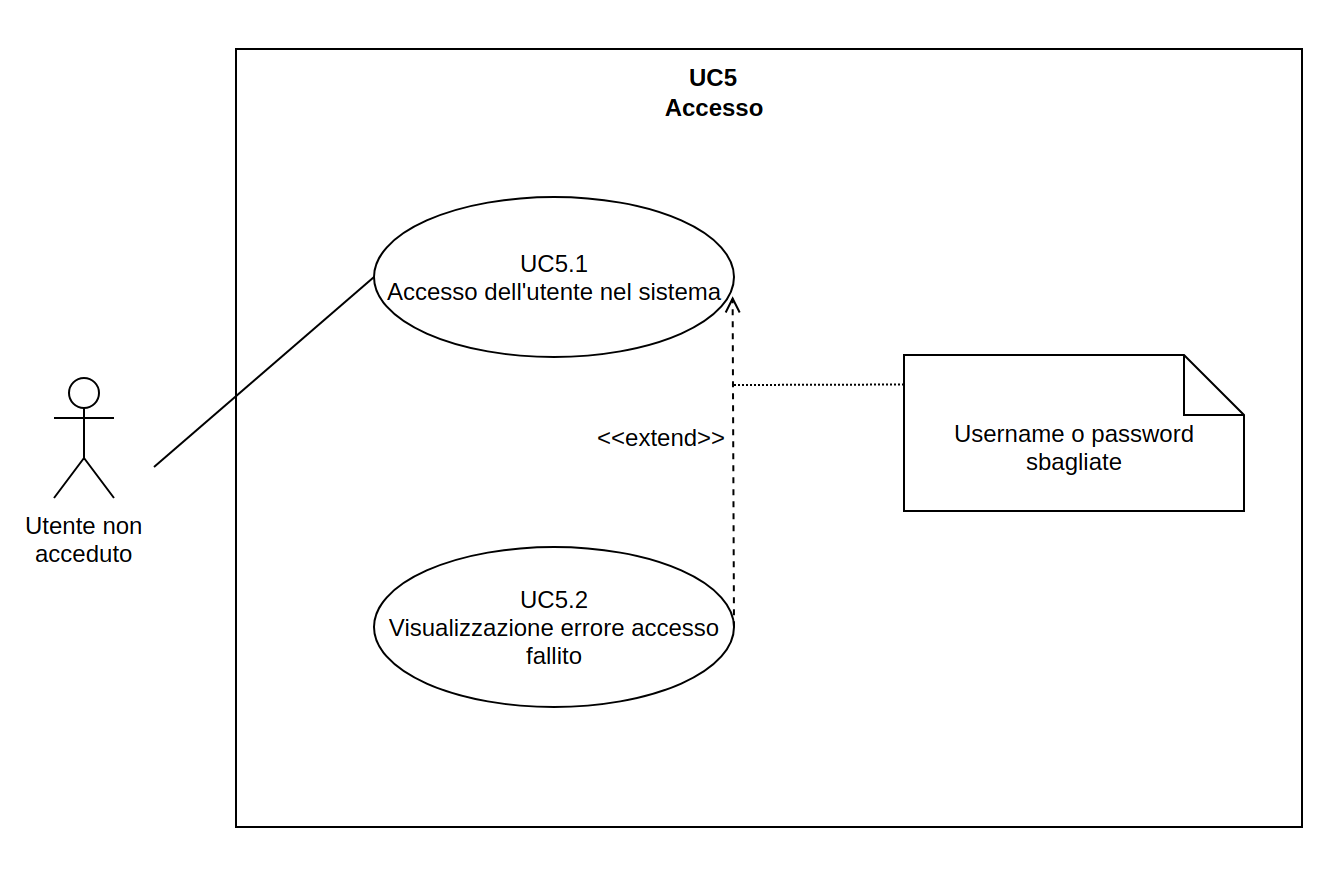
\includegraphics[width=\columnwidth]{img/UC5.png}\\
			\caption{UC\theuccount-GP - Modifica utente}
		\end{figure}
	\begin{itemize}
		\item \textbf{Codice}: UC\theuccount-GP.
		\item \textbf{Titolo}: modifica utente.
		\item \textbf{Attori primari}: utente acceduto.
		\item \textbf{Descrizione}: l’utente vuole modificare le informazioni relative a un utente.
		\item \textbf{Precondizione}: l'utente acceduto vuole modificare un utente già presente.
		\item \textbf{Postcondizione}: i campi dell'utente sono stati modificati correttamente.
		\item \textbf{Scenario Principale}:
		\begin{enumerate}
			\item Utente acceduto procede alla modifica di un utente.
		\end{enumerate}
	\end{itemize}

	\paragraph{UC\theuccount.1-GP - Selezione ID utente}
		\begin{figure}[H]
			\centering
			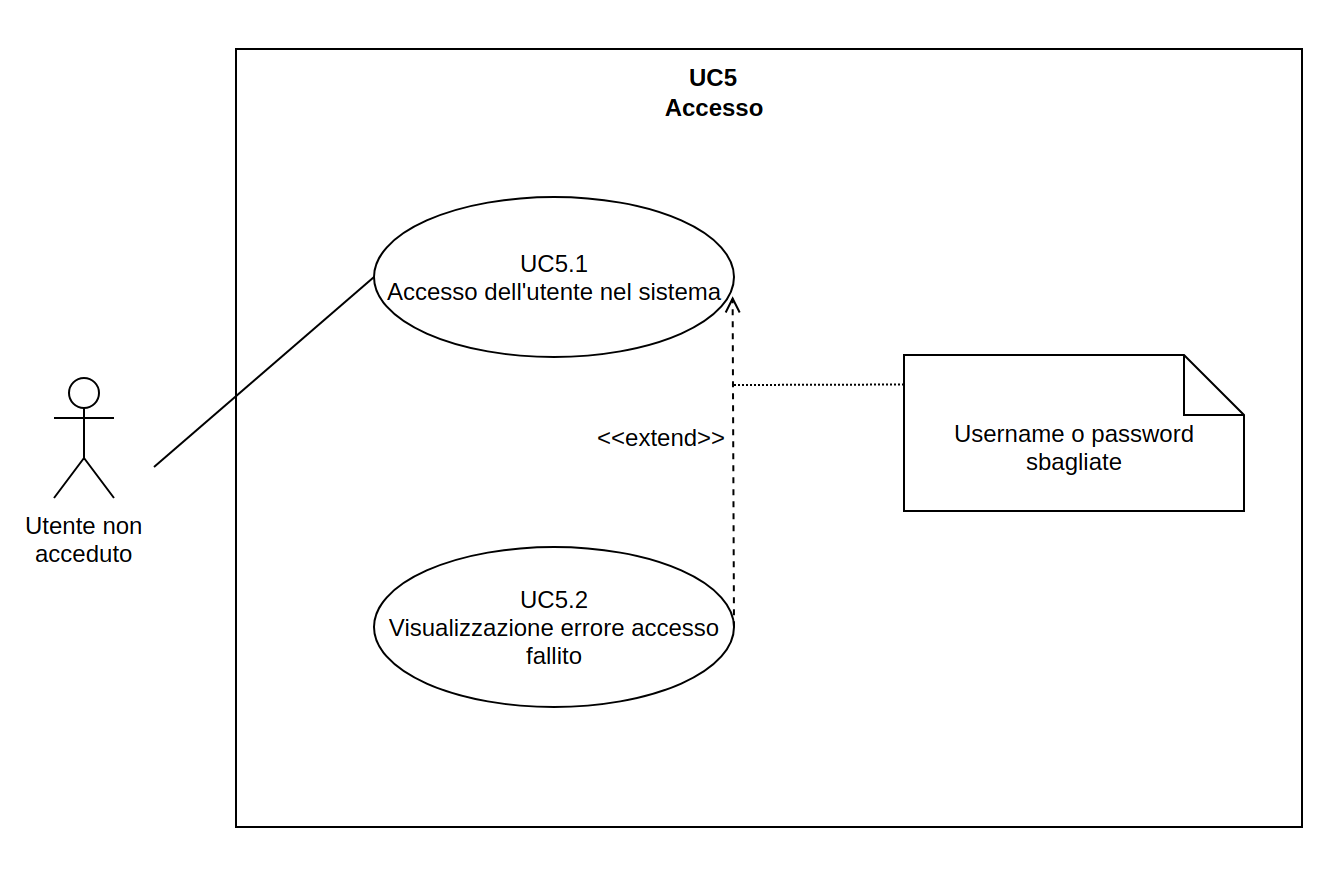
\includegraphics[width=\columnwidth]{img/UC5.png}\\
			\caption{UC\theuccount.1-GP - Selezione ID utente}
		\end{figure}
		\begin{itemize}
			\item \textbf{Codice}: UC\theuccount.1-GP.
			\item \textbf{Titolo}: selezione ID utente.
			\item \textbf{Attori primari}: utente acceduto.
			\item \textbf{Descrizione}: l'utente ha aggiunto il nuovo nome dell'utente che vuole modificare.
			\item \textbf{Precondizione}: l'utente acceduto vuole modificare un utente già presente.
			\item \textbf{Postcondizione}: l'ID utente è stato inserito.
			\item \textbf{Scenario Principale}:
			\begin{enumerate}
				\item Utente acceduto procede all'inserimento dell'ID utente da modificare.
			\end{enumerate}
			\item \textbf{Estensioni}:
			\begin{itemize}
				\item Errore user ID inesistente[UC15.2-GP]
			\end{itemize}
		\end{itemize}
	
		\subparagraph{UC\theuccount.1.1-GP - Modifica utente avvenuta con successo}
			\begin{figure}[H]
				\centering
				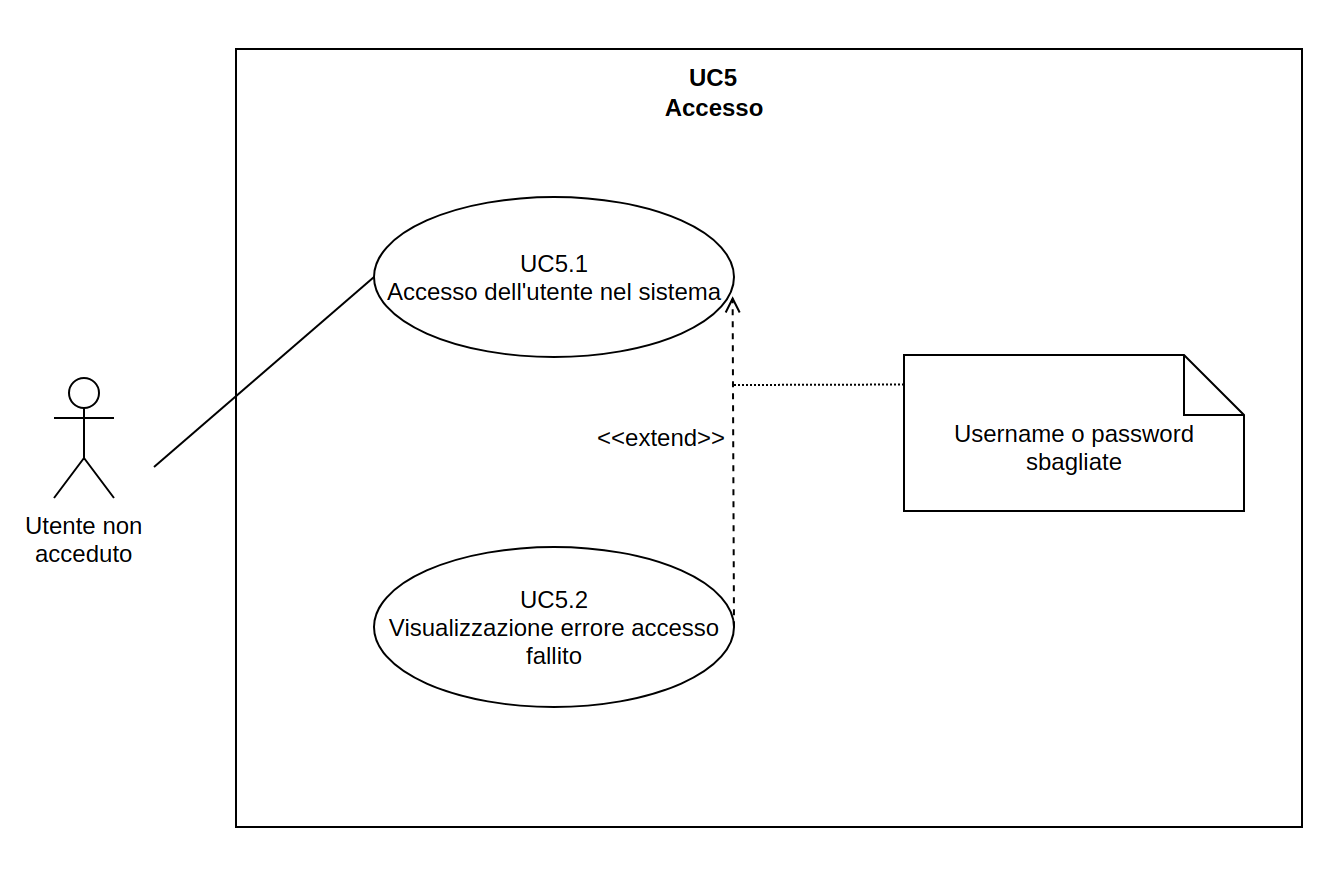
\includegraphics[width=\columnwidth]{img/UC5.png}\\
				\caption{UC\theuccount.1.1-GP - Modifica utente avvenuta con successo}
			\end{figure}
			\begin{itemize}
				\item \textbf{Codice}: UC\theuccount.1.1-GP.
				\item \textbf{Titolo}: modifica utente avvenuta con successo.
				\item \textbf{Attori primari}: utente acceduto.
				\item \textbf{Descrizione}: l'ID utente è presente nel sistema e ne vengono modificati i relativi campi con successo.
				\item \textbf{Precondizione}: l'utente acceduto vuole modificare un utente già presente.
				\item \textbf{Postcondizione}: l'utente è stato modificato con successo.
				\item \textbf{Scenario Principale}:
				\begin{enumerate}
					\item Utente viene modificato con successo.
				\end{enumerate}
			\end{itemize}
		
			\subsubparagraph{UC\theuccount.1.1.1-GP - Inserimento del nuovo nome}
				\begin{figure}[H]
					\centering
					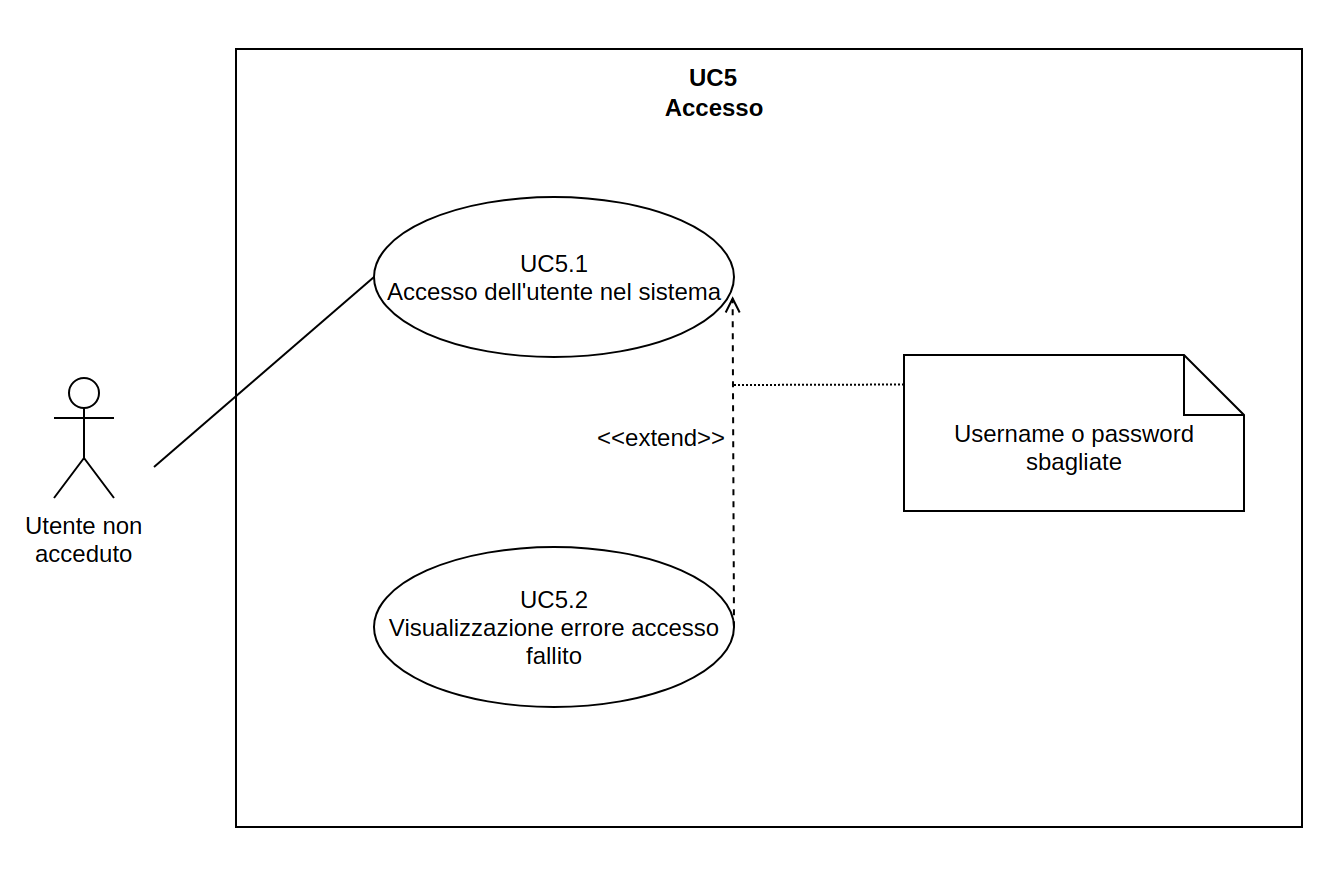
\includegraphics[width=\columnwidth]{img/UC5.png}\\
					\caption{UC\theuccount.1.1.1-GP - Inserimento del nuovo nome}
				\end{figure}
				\begin{itemize}
					\item \textbf{Codice}: UC\theuccount.1.1.1-GP.
					\item \textbf{Titolo}: inserimento del nuovo nome.
					\item \textbf{Attori primari}: utente acceduto.
					\item \textbf{Descrizione}: l'utente aggiunge il nuovo nome relativo all'ID utente inserito che vuole modificare.
					\item \textbf{Precondizione}: l'utente acceduto vuole modificare un utente già presente.
					\item \textbf{Postcondizione}: il nome è stato inserito.
					\item \textbf{Scenario Principale}:
					\begin{enumerate}
						\item Utente acceduto inserisce il nuovo nome dell'utente che vuole modificare.
					\end{enumerate}
				\end{itemize}
			
			\subsubparagraph{UC\theuccount.1.1.2-GP - Inserimento del nuovo cognome}
				\begin{figure}[H]
					\centering
					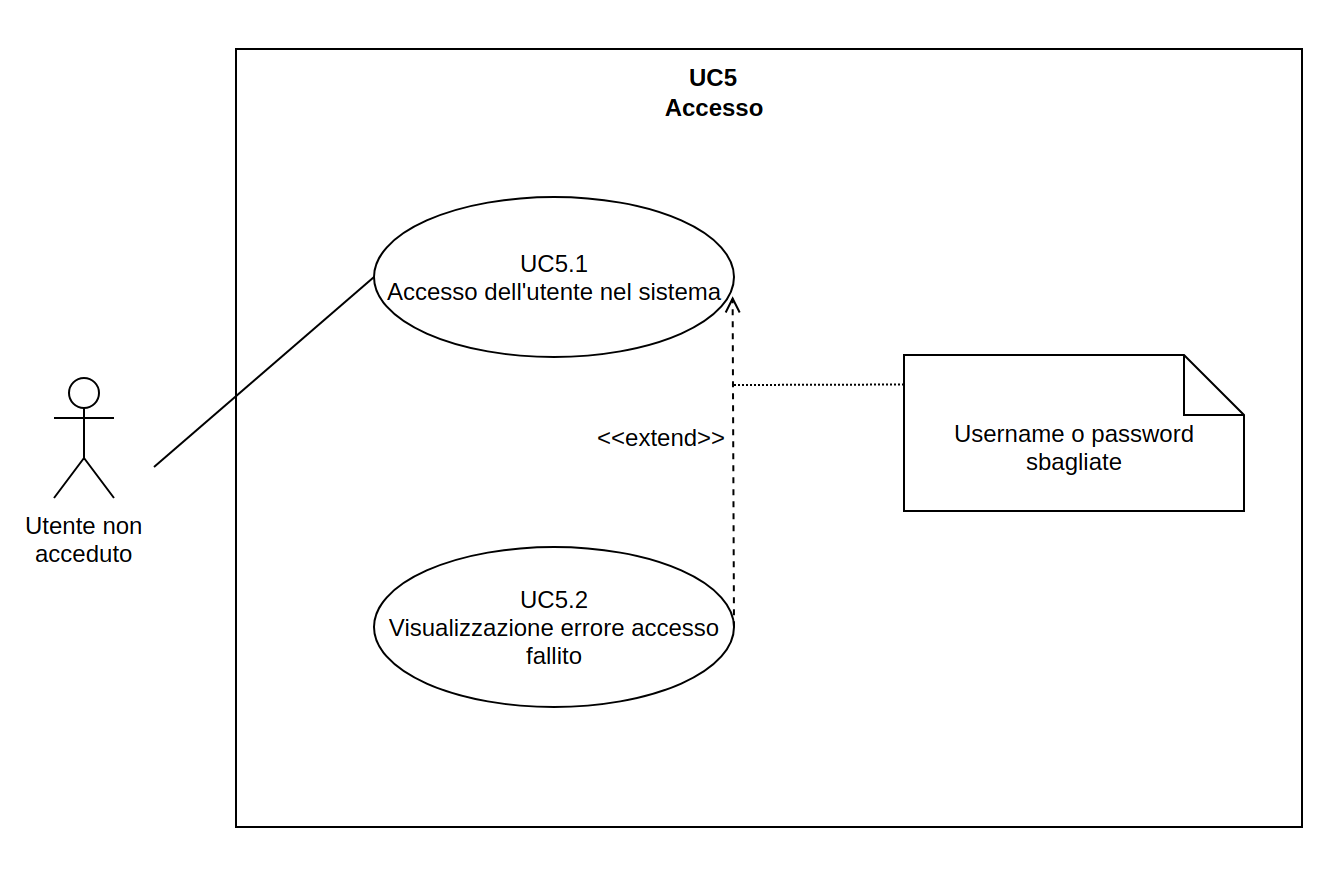
\includegraphics[width=\columnwidth]{img/UC5.png}\\
					\caption{UC\theuccount.1.1.2-GP - Inserimento del nuovo cognome}
				\end{figure}
				\begin{itemize}
					\item \textbf{Codice}: UC\theuccount.1.1.2-GP.
					\item \textbf{Titolo}: inserimento del nuovo cognome.
					\item \textbf{Attori primari}: utente acceduto.
					\item \textbf{Descrizione}: l'utente aggiunge il nuovo cognome relativo all'ID utente inserito che vuole modificare.
					\item \textbf{Precondizione}: l'utente acceduto vuole modificare un utente già presente.
					\item \textbf{Postcondizione}: il cognome è stato inserito.
					\item \textbf{Scenario Principale}:
					\begin{enumerate}
						\item Utente acceduto inserisce il nuovo cognome dell'utente che vuole modificare.
					\end{enumerate}
				\end{itemize}
			
			\subsubparagraph{UC\theuccount.1.1.3-GP - Inserimento del nuovo contatto Email}
				\begin{figure}[H]
					\centering
					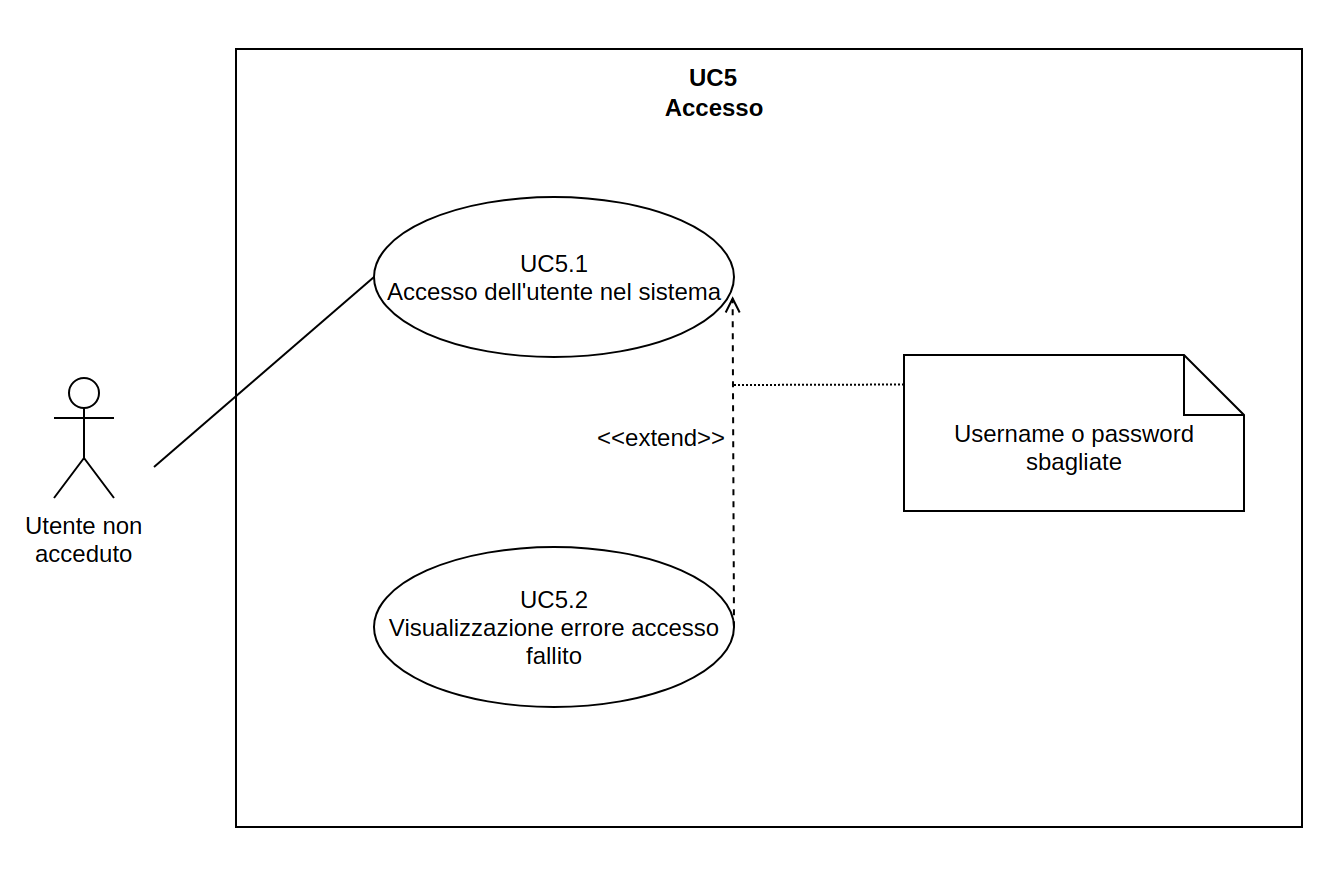
\includegraphics[width=\columnwidth]{img/UC5.png}\\
					\caption{UC\theuccount.1.1.3-GP - Inserimento del nuovo contatto Email}
				\end{figure}
				\begin{itemize}
					\item \textbf{Codice}: UC\theuccount.1.1.3-GP.
					\item \textbf{Titolo}: inserimento del nuovo contatto Email.
					\item \textbf{Attori primari}: utente acceduto.
					\item \textbf{Descrizione}: l'utente aggiunge il nuovo contatto Email relativo all'ID utente inserito che vuole modificare.
					\item \textbf{Precondizione}: l'utente acceduto vuole modificare un utente già presente.
					\item \textbf{Postcondizione}: il contatto Email è stato inserito.
					\item \textbf{Scenario Principale}:
					\begin{enumerate}
						\item Utente acceduto inserisce il nuovo contatto Email dell'utente che vuole modificare.
					\end{enumerate}
				\end{itemize}
			
			\subsubparagraph{UC\theuccount.1.1.4-GP - Inserimento del nuovo contatto Telegram}
				\begin{figure}[H]
					\centering
					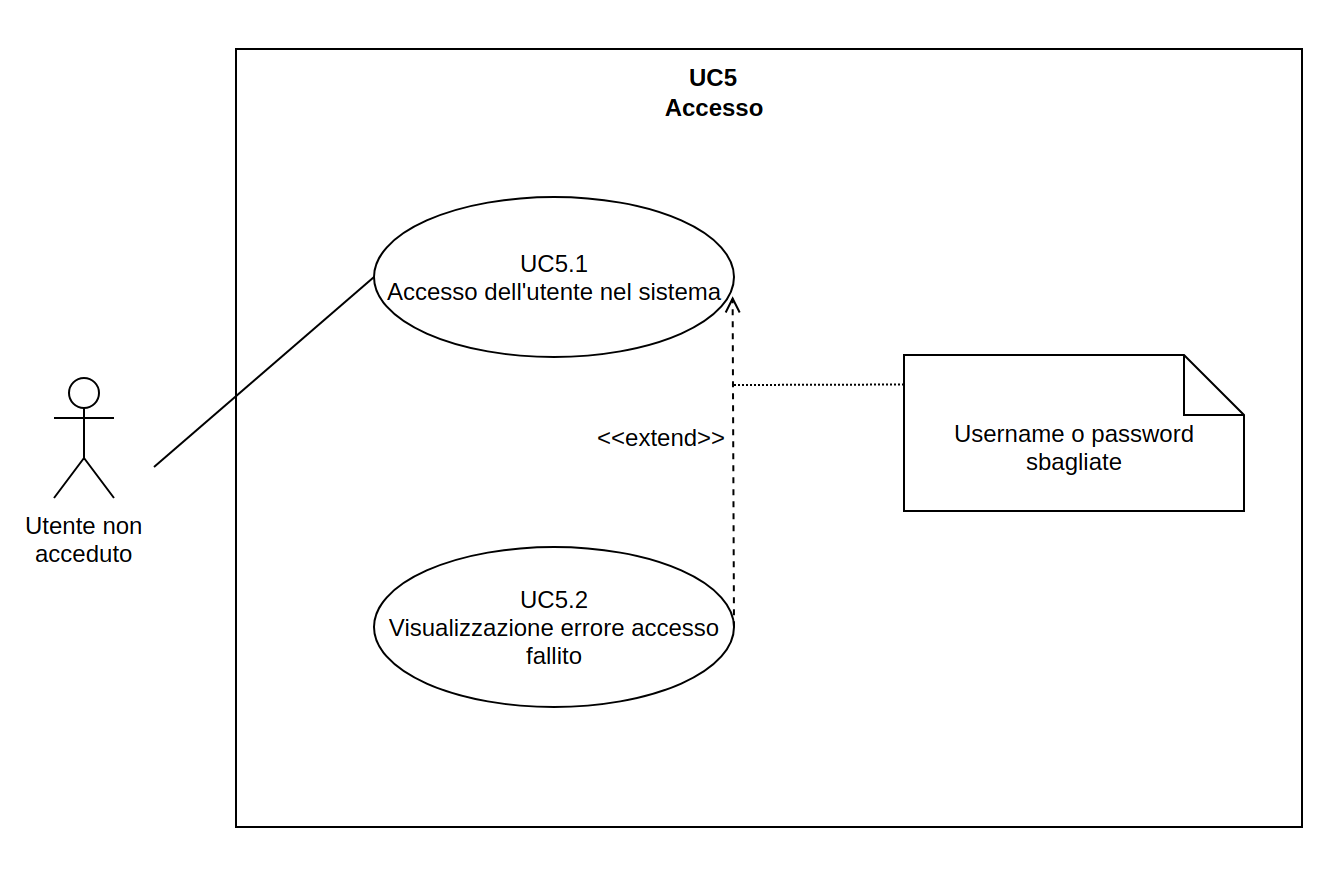
\includegraphics[width=\columnwidth]{img/UC5.png}\\
					\caption{UC\theuccount.1.1.4-GP - Inserimento del nuovo contatto Telegram}
				\end{figure}
				\begin{itemize}
					\item \textbf{Codice}: UC\theuccount.1.1.4-GP.
					\item \textbf{Titolo}: inserimento del nuovo contatto Telegram.
					\item \textbf{Attori primari}: utente acceduto.
					\item \textbf{Descrizione}: l'utente aggiunge il nuovo contatto Telegram relativo all'ID utente inserito che vuole modificare.
					\item \textbf{Precondizione}: l'utente acceduto vuole modificare un utente già presente.
					\item \textbf{Postcondizione}: il contatto Telegram è stato inserito.
					\item \textbf{Scenario Principale}:
					\begin{enumerate}
						\item Utente acceduto inserisce il nuovo contatto Telegram dell'utente che vuole modificare.
					\end{enumerate}
				\end{itemize}
		
	\paragraph{UC\theuccount.2-GP - Errore ID utente inesistente}
		\begin{figure}[H]
			\centering
			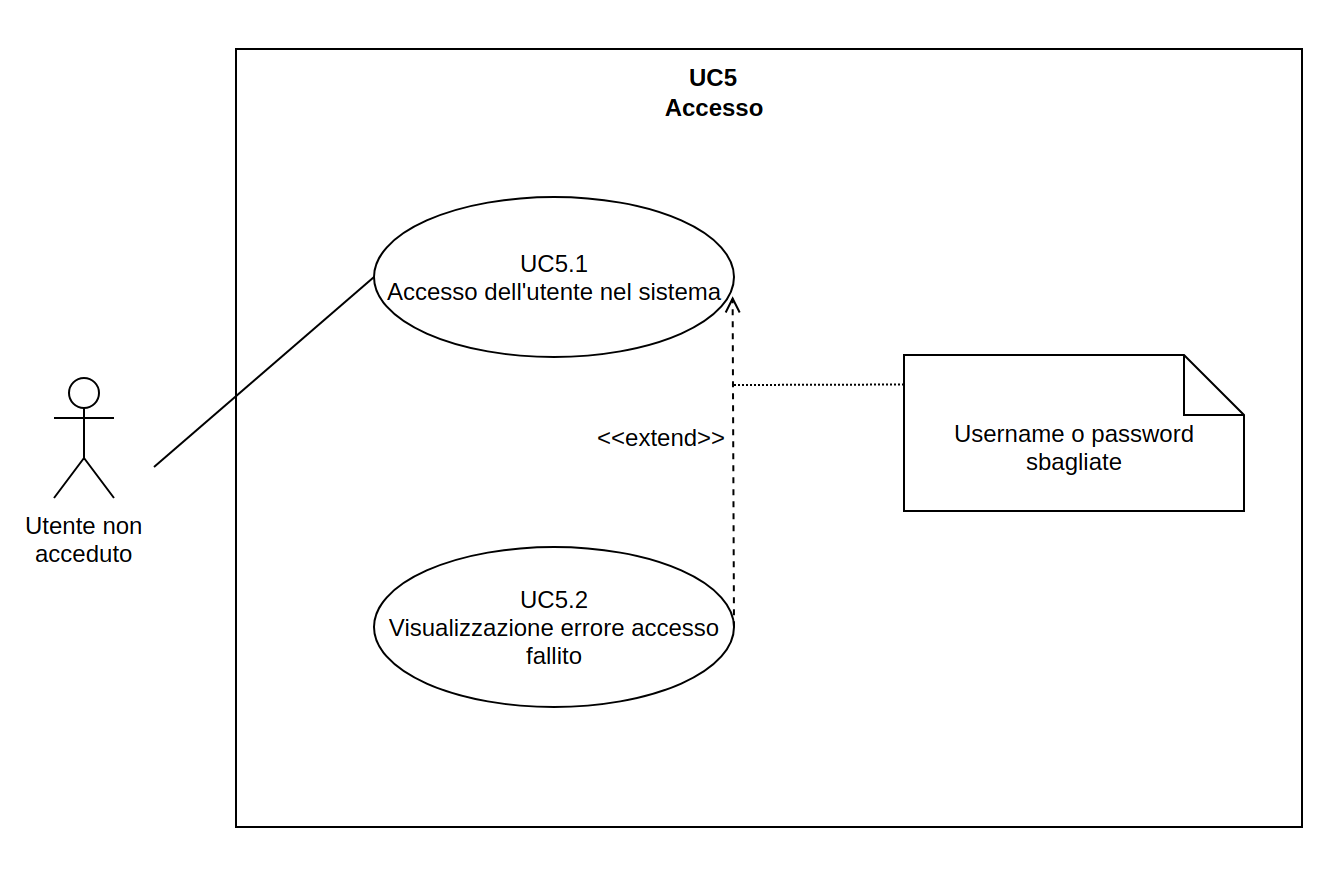
\includegraphics[width=\columnwidth]{img/UC5.png}\\
			\caption{UC\theuccount.2-GP - Errore ID utente inesistente}
		\end{figure}
		\begin{itemize}
			\item \textbf{Codice}: UC\theuccount.2-GP.
			\item \textbf{Titolo}: errore ID utente inesistente.
			\item \textbf{Attori primari}: utente acceduto.
			\item \textbf{Descrizione}:  l’utente viene avvisato che ha inserito un'ID utente errato.
			\item \textbf{Precondizione}: l'utente acceduto vuole modificare un utente già presente.
			\item \textbf{Postcondizione}: il sistema comunica all’utilizzatore l’errore.
			\item \textbf{Scenario Principale}:
			\begin{enumerate}
				\item L'utente ha inserito un ID utente errato e il sistema comunica all’utilizzatore l’errore.
			\end{enumerate}
		\end{itemize}

\stepcounter{uccount}

\subsubsection{UC\theuccount-GP - Aggiunta preferenze}
		\begin{figure}[H]
			\centering
				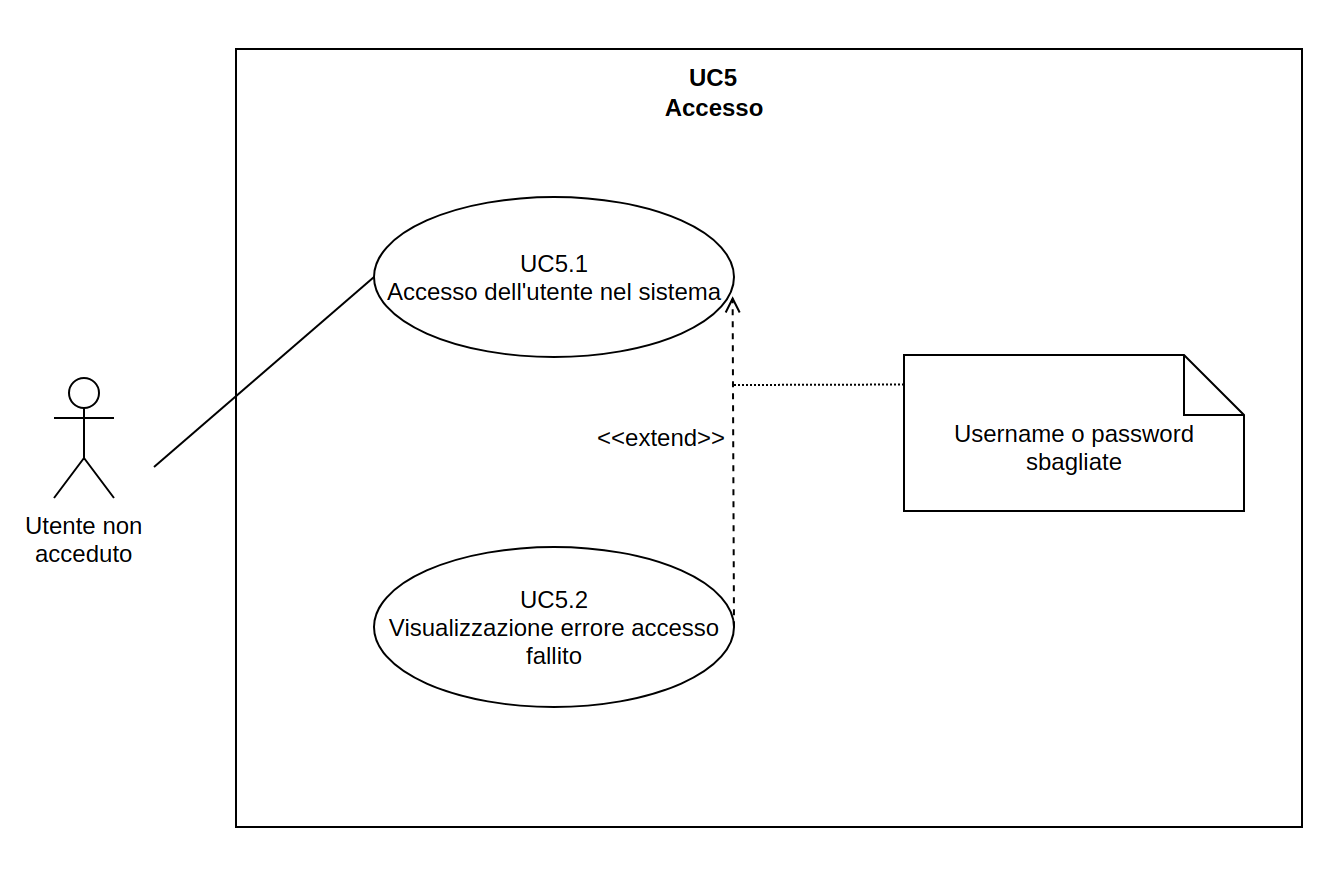
\includegraphics[width=\columnwidth]{img/UC5.png}\\
			\caption{UC\theuccount-GP - Aggiunta preferenze}
		\end{figure}
	\begin{itemize}
		\item \textbf{Codice}: UC\theuccount-GP.
		\item \textbf{Titolo}: aggiunta preferenze.
		\item \textbf{Attori primari}: utente acceduto.
		\item \textbf{Descrizione}: l’utente, date le varie opzioni per configurare Butterfly, aggiunge una
		preferenza tra Topic, giorni di calendario, piattaforma di messaggistica (Telegram o e-mail)
		preferita e la persona di fiducia che lo può sostituire.
		\item \textbf{Precondizione}: l’utente ha acceduto con le sue credenziali corrette nel sistema e non
		ha già selezionato tutte le preferenze possibili proposte da Butterfly.
		\item \textbf{Postcondizione}: la nuova configurazione contiene una o più preferenze in aggiunta rispetto a quella precedente.
		\item \textbf{Scenario Principale}:
		\begin{enumerate}
			\item Utente acceduto procede all'aggiunta di una o più preferenze.
		\end{enumerate}
	\end{itemize}


	\paragraph{UC\theuccount.1-GP - Iscrizione Topic}
		\begin{figure}[H]
			\centering
			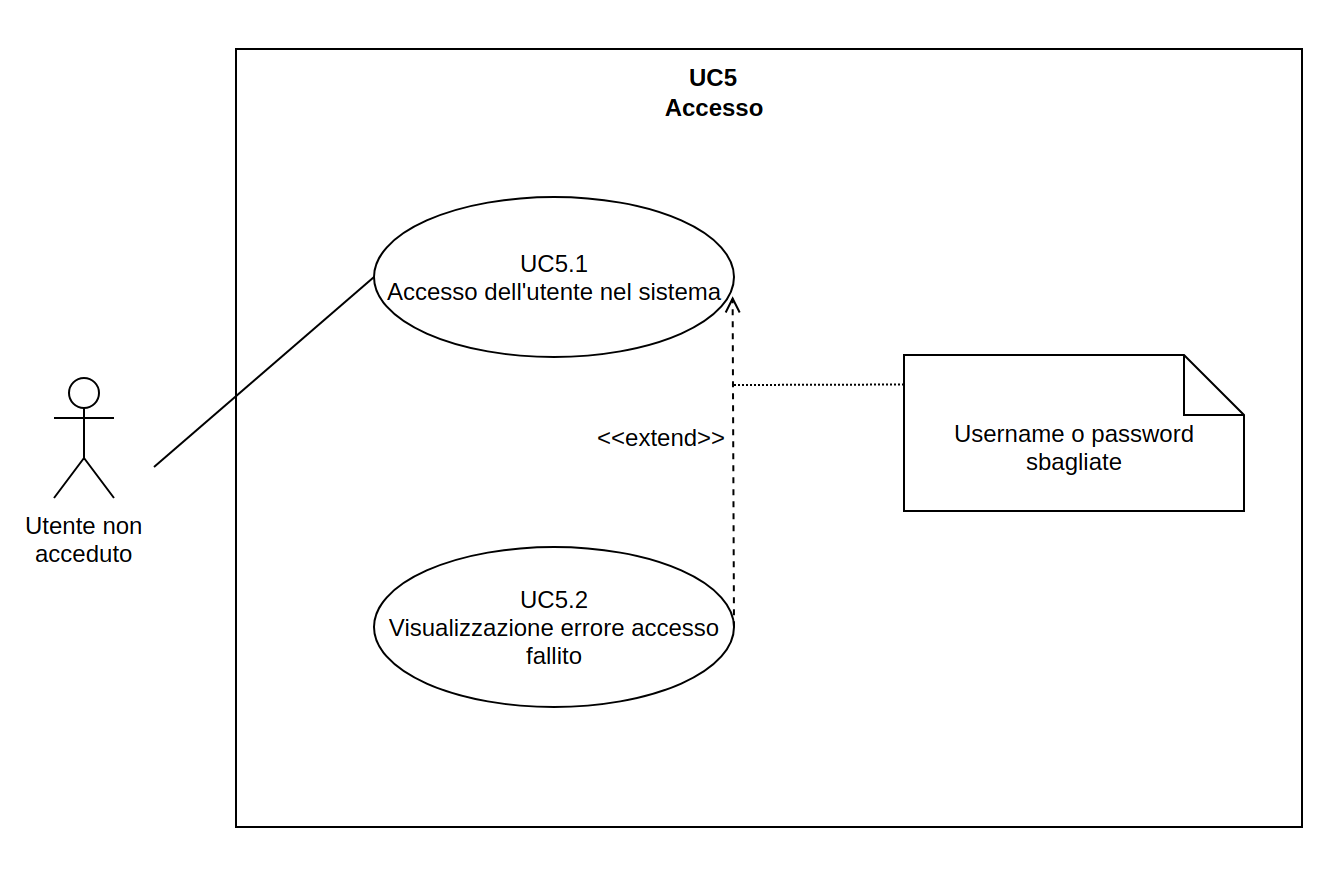
\includegraphics[width=\columnwidth]{img/UC5.png}\\
			\caption{UC\theuccount.1-GP - Iscrizione Topic}
		\end{figure}
		\begin{itemize}
			\item \textbf{Codice}: UC\theuccount.1-GP.
			\item \textbf{Titolo}: iscrizione Topic.
			\item \textbf{Attori primari}: utente acceduto.
			\item \textbf{Descrizione}: data la lista di Topic presenti, l’utente ne seleziona uno o
			più a cui è interessato, ricevendone una notifica. I Topic sono divisi per categoria e
			comprendono etichette, progetto a cui sono legate e l'applicazione di provenienza: Redmine o GitLab.
			\item \textbf{Precondizione}: l’utente ha acceduto correttamente nel sistema e non ha già
			selezionato tutti i Topic possibili proposti da Butterfly.
			\item \textbf{Postcondizione}: il numero di Topic a cui è interessato l’utente è aumentato.
			\item \textbf{Scenario Principale}:
			\begin{enumerate}
				\item Utente acceduto procede all'iscrizione di uno o più Topic.
			\end{enumerate}
		\end{itemize}
	
		\paragraph{UC\theuccount.2-GP - Aggiunta dei giorni di indisponibilità nel calendario}
			\begin{figure}[H]
				\centering
				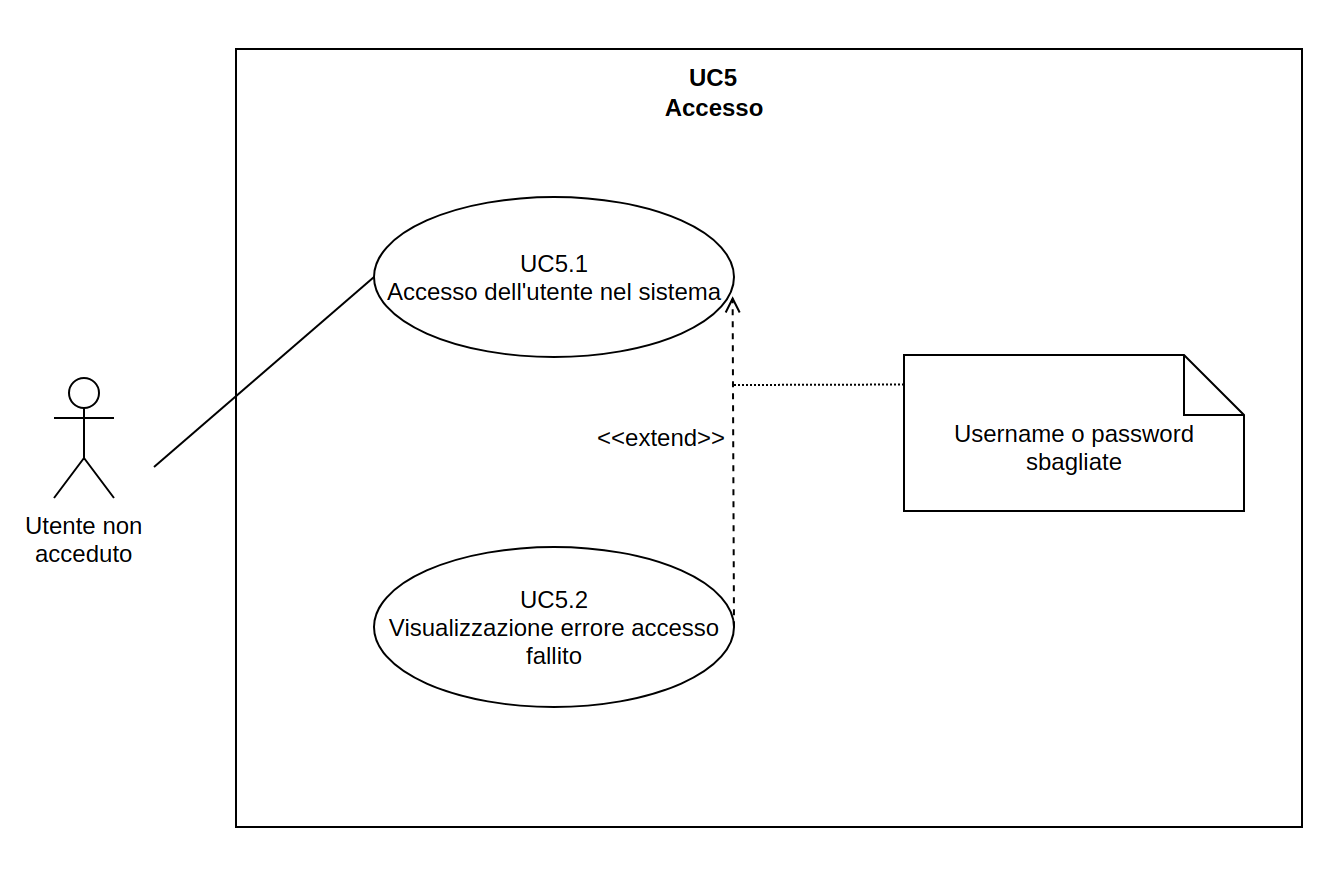
\includegraphics[width=\columnwidth]{img/UC5.png}\\
				\caption{UC\theuccount.2-GP - Aggiunta dei giorni di indisponibilità nel calendario}
			\end{figure}
			\begin{itemize}
				\item \textbf{Codice}: UC\theuccount.2-GP.
				\item \textbf{Titolo}: aggiunta dei giorni di indisponibilità nel calendario.
				\item \textbf{Attori primari}: utente acceduto.
				\item \textbf{Descrizione}: dato il calendario lavorativo, l’utente aggiunge uno o più
				giorni in cui non è reperibile e non vuole ricevere notifiche.
				\item \textbf{Precondizione}: l’utente ha acceduto correttamente nel sistema e non
				ha già selezionato tutti i giorni di indisponibilità.
				\item \textbf{Postcondizione}: il numero di giorni in cui l’utente non si rende disponibile è aumentato.
				\item \textbf{Scenario Principale}:
				\begin{enumerate}
					\item Utente acceduto procede all'inserimento di uno o più giorni di indisponibilità.
				\end{enumerate}
			\end{itemize}
		
			\paragraph{UC\theuccount.3-GP - Aggiunta della piattaforma di messaggistica preferita}
				\begin{figure}[H]
					\centering
					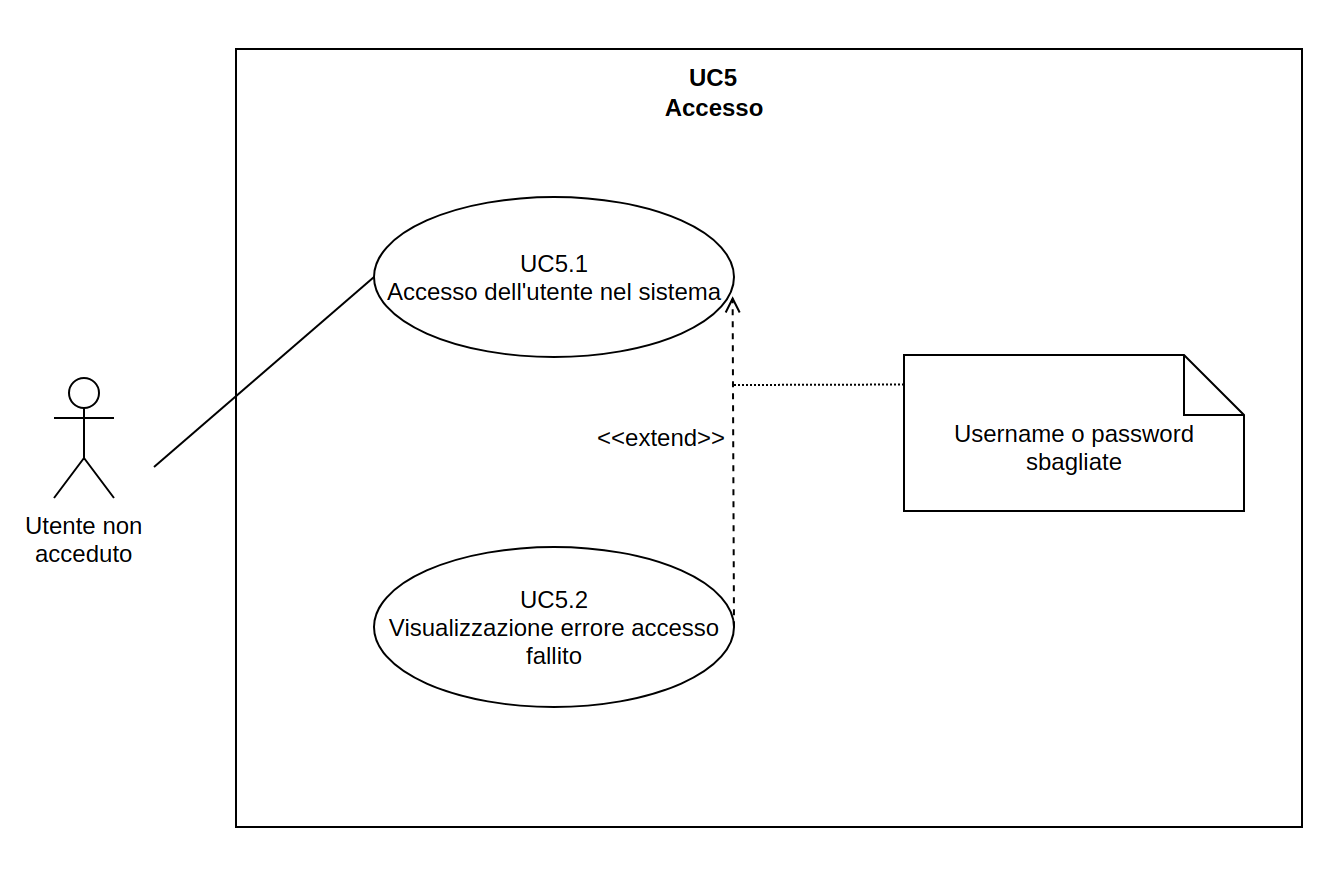
\includegraphics[width=\columnwidth]{img/UC5.png}\\
					\caption{UC\theuccount.3-GP - Aggiunta della piattaforma di messaggistica preferita}
				\end{figure}
				\begin{itemize}
					\item \textbf{Codice}: UC\theuccount.3-GP.
					\item \textbf{Titolo}: aggiunta della piattaforma di messaggistica preferita.
					\item \textbf{Attori primari}: utente acceduto.
					\item \textbf{Descrizione}: l’utente aggiunge la sua preferenza tra Telegram e email dove
					vuole ricevere le notifiche.
					\item \textbf{Precondizione}: l’utente ha acceduto correttamente nel sistema e non ha
					già selezionato tutte le piattaforme di messaggistica possibili proposte da Butterfly.
					\item \textbf{Postcondizione}: il numero di piattaforme di messaggistica selezionate dall’utente è aumentato.
					\item \textbf{Scenario Principale}:
					\begin{enumerate}
						\item Utente acceduto procede all'aggiunta di una o più piattaforme di messaggistica.
					\end{enumerate}
				\end{itemize}
			
			\paragraph{UC\theuccount.4-GP - Aggiunta persona di fiducia}
				\begin{figure}[H]
					\centering
					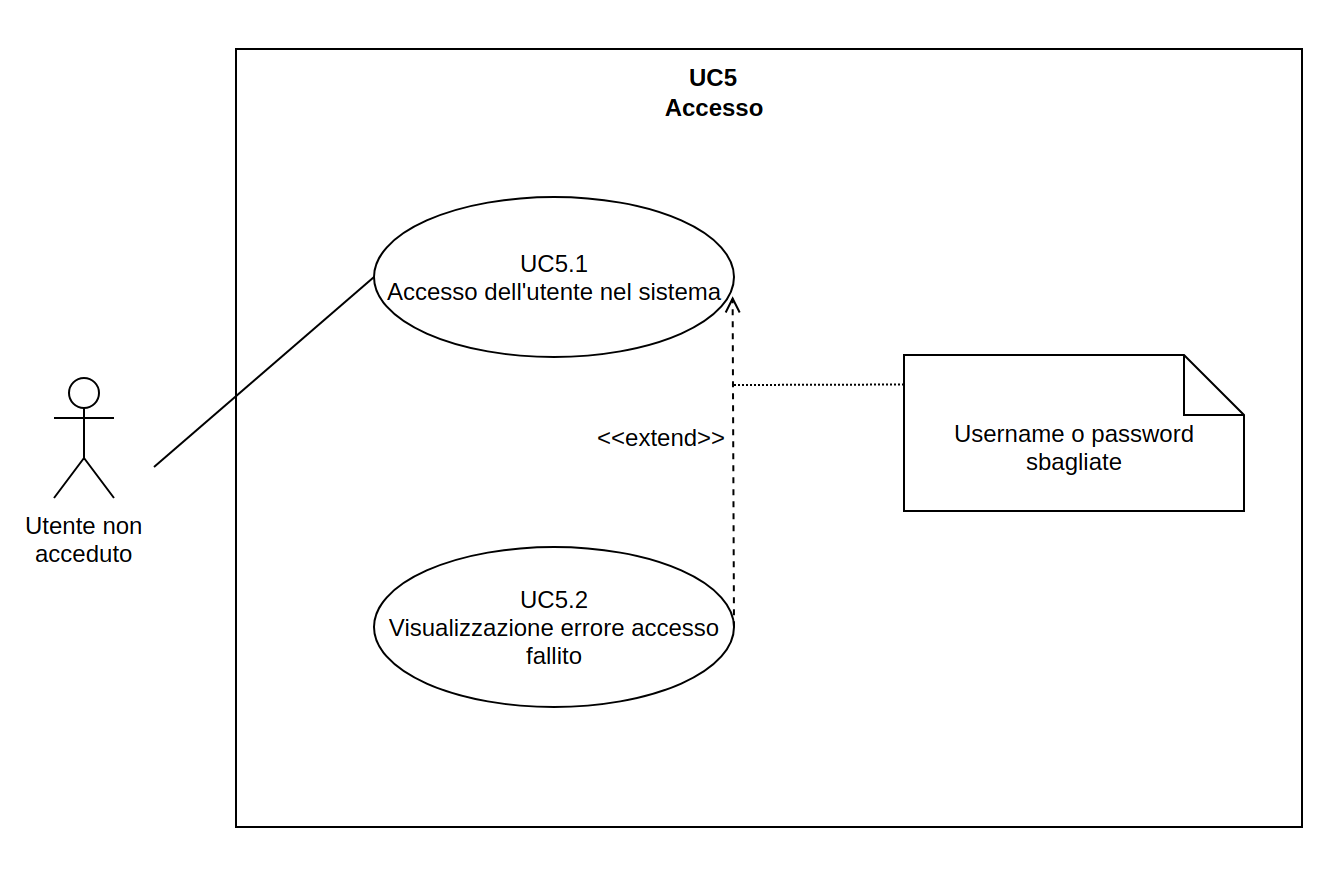
\includegraphics[width=\columnwidth]{img/UC5.png}\\
					\caption{UC\theuccount.4-GP - Aggiunta persona di fiducia}
				\end{figure}
				\begin{itemize}
					\item \textbf{Codice}: UC\theuccount.4-GP.
					\item \textbf{Titolo}: aggiunta persona di fiducia.
					\item \textbf{Attori primari}: utente acceduto.
					\item \textbf{Descrizione}: l’utente acceduto aggiunge l'utente legato a un ID di sua preferenza a
					cui inoltrare i messaggi in caso di indisponibilità.
					\item \textbf{Precondizione}: l’utente ha acceduto con le sue credenziali corrette nel
					sistema e non ha già selezionato la persona a cui inoltrare le notifiche.
					\item \textbf{Postcondizione}: la preferenza viene aggiunta correttamente.
					\item \textbf{Scenario Principale}:
					\begin{enumerate}
						\item Utente acceduto procede all'aggiunta della sua persona di fiducia.
					\end{enumerate}
					\item \textbf{Estensioni}:
					\begin{enumerate}
						\item Errore ID persona di fiducia inesistente[UC16.5-GP].
					\end{enumerate}
				\end{itemize}
			
			\paragraph{UC\theuccount.5-GP - Errore ID persona di fiducia inesistente}
				\begin{figure}[H]
					\centering
					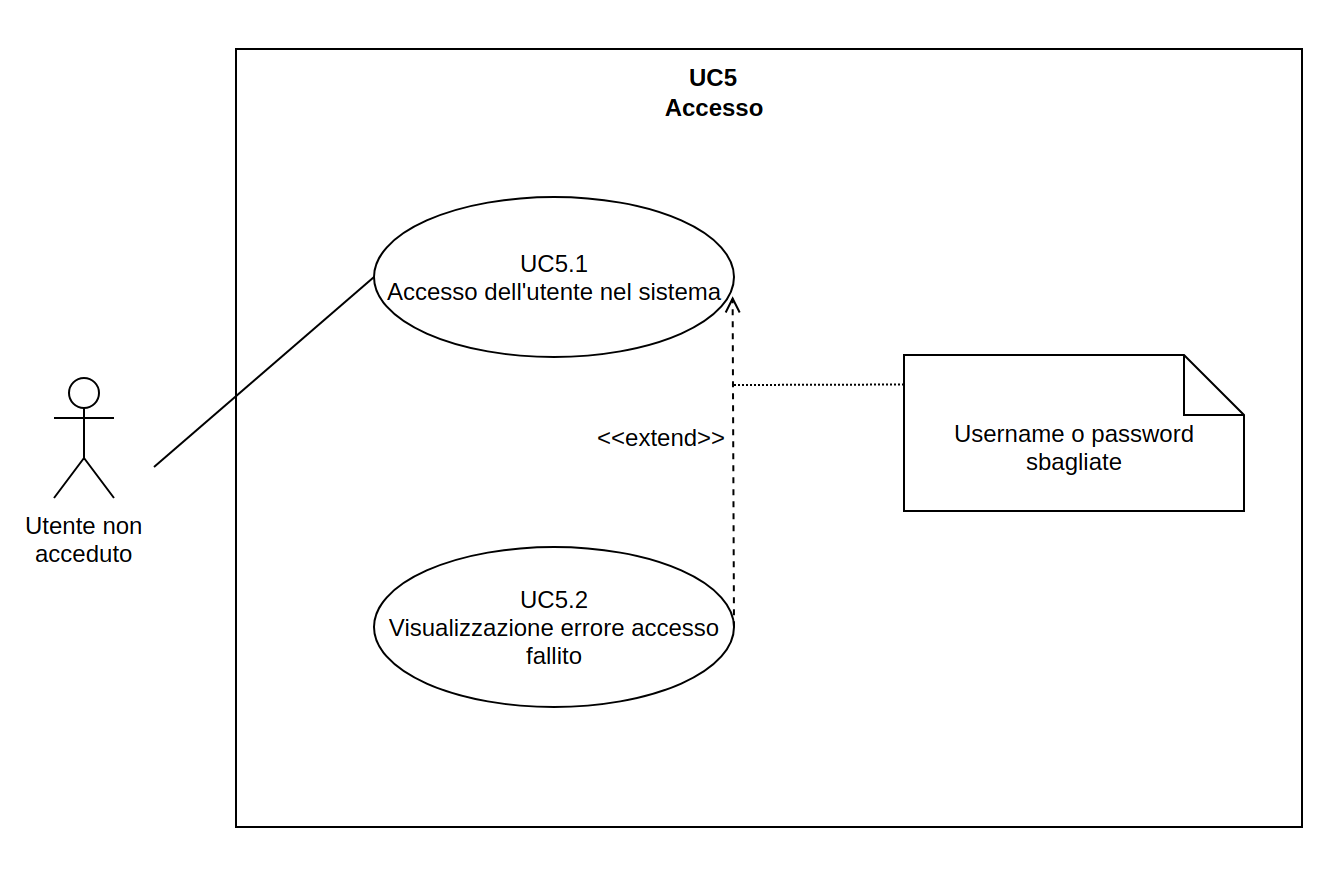
\includegraphics[width=\columnwidth]{img/UC5.png}\\
					\caption{UC\theuccount.5-GP - Errore ID persona di fiducia inesistente}
				\end{figure}
				\begin{itemize}
					\item \textbf{Codice}: UC\theuccount.5-GP.
					\item \textbf{Titolo}: errore ID persona di fiducia inesistente.
					\item \textbf{Attori primari}: utente acceduto.
					\item \textbf{Descrizione}: l’utente viene avvisato che ha inserito un ID utente errato.
					\item \textbf{Precondizione}: l’utente ha acceduto con le sue credenziali corrette nel
					sistema e non ha già selezionato la persona a cui inoltrare le notifiche.
					\item \textbf{Postcondizione}: il sistema comunica all’utilizzatore l’errore di preferenza.
					\item \textbf{Scenario Principale}:
					\begin{enumerate}
						\item Utente acceduto procede all'aggiunta della sua persona di fiducia ma questa non esiste e
						visualizza l'errore.
					\end{enumerate}
				\end{itemize}
			
			\paragraph{UC\theuccount.6-GP - Aggiunta keyword per i push di GitLab}
				\begin{figure}[H]
					\centering
					\includegraphics[width=\columnwidth]{img/UC5.png}\\
					\caption{UC\theuccount.6-GP - Aggiunta keyword per i push di GitLab}
				\end{figure}
				\begin{itemize}
					\item \textbf{Codice}: UC\theuccount.6-GP.
					\item \textbf{Titolo}: aggiunta keyword per i push di GitLab.
					\item \textbf{Attori primari}: utente acceduto.
					\item \textbf{Descrizione}: l’utente aggiunge le keyword che vuole che siano contenute
					nei messaggi di commit dei push di cui vuole ricevere la notifica.
					\item \textbf{Precondizione}: l’utente ha acceduto con le sue credenziali corrette nel sistema.
					\item \textbf{Postcondizione}: nelle nuove configurazioni dell'utente selezionato sono
					presenti una o più nuove keyword per ricevere notifiche da push di GitLab.
					\item \textbf{Scenario Principale}:
					\begin{enumerate}
						\item Utente acceduto procede all'aggiunta di una o più nuove keyword.
					\end{enumerate}
				\end{itemize}

\stepcounter{uccount}

\subsubsection{UC\theuccount-GP - Rimozione preferenze}
		\begin{figure}[H]
			\centering
				\includegraphics[width=\columnwidth]{img/UC5.png}\\
			\caption{UC\theuccount-GP - Rimozione preferenze}
		\end{figure}
	\begin{itemize}
		\item \textbf{Codice}: UC\theuccount-GP.
		\item \textbf{Titolo}: rimozione preferenze.
		\item \textbf{Attori primari}: utente acceduto.
		\item \textbf{Descrizione}: l’utente, dopo aver selezionato delle preferenze dalle opzioni
		di configurazione, ne rimuove una o più. Le preferenze consistono in Topic, date di calendario,
		piattaforma di messaggistica (Telegram e email) e persona di fiducia che lo può sostituire.
		\item \textbf{Precondizione}: l’utente ha eseguito l'accesso nel sistema ed è presente almeno
		una preferenza selezionata tra quelle proposte da Butterfly.
		\item \textbf{Postcondizione}: la nuova configurazione contiene una o più preferenze in meno rispetto
		a quella precedente.
		\item \textbf{Scenario Principale}:
		\begin{enumerate}
			\item Utente acceduto procede alla rimozione di una o più preferenze.
		\end{enumerate}
	\end{itemize}


	\paragraph{UC\theuccount.1-GP - Disiscrizione Topic}
		\begin{figure}[H]
			\centering
			\includegraphics[width=\columnwidth]{img/UC5.png}\\
			\caption{UC\theuccount.1-GP - Disiscrizione Topic}
		\end{figure}
		\begin{itemize}
			\item \textbf{Codice}: UC\theuccount.1-GP.
			\item \textbf{Titolo}: disiscrizione Topic.
			\item \textbf{Attori primari}: utente acceduto.
			\item \textbf{Descrizione}: l’utente si disiscrive da uno o più Topic dai quali prima riceveva
			delle notifiche.
			\item \textbf{Precondizione}: l’utente ha acceduto correttamente nel sistema e non ha già
			selezionato tutti i Topic possibili proposti da Butterfly.
			\item \textbf{Postcondizione}: il numero di Topic a cui è iscritto l’utente è diminuito.
			\item \textbf{Scenario Principale}:
			\begin{enumerate}
				\item Utente acceduto procede alla disiscrizione di uno o più Topic.
			\end{enumerate}
		\end{itemize}
		
		\paragraph{UC\theuccount.2-GP - Rimozione di uno o più giorni di irreperibilità nel calendario}
		\begin{figure}[H]
			\centering
			\includegraphics[width=\columnwidth]{img/UC5.png}\\
			\caption{UC\theuccount.2-GP - Rimozione di uno o più giorni di irreperibilità nel calendario}
		\end{figure}
		\begin{itemize}
			\item \textbf{Codice}: UC\theuccount.2-GP.
			\item \textbf{Titolo}: rimozione di uno o più giorni di irreperibilità nel calendario.
			\item \textbf{Attori primari}: utente acceduto.
			\item \textbf{Descrizione}: l’utente rimuove i giorni di calendario in cui precedentemente
			non era reperibile, tornando disponibile.
			\item \textbf{Precondizione}: l’utente ha acceduto correttamente nel sistema ed è presente
			almeno un giorno di calendario selezionato tra quelli proposti da Butterfly.
			\item \textbf{Postcondizione}: il numero di giorni di calendario in cui l’utente non è reperibile è diminuito.
			\item \textbf{Scenario Principale}:
			\begin{enumerate}
				\item Utente acceduto procede alla rimozione di uno o più giorni di irreperibilità.
			\end{enumerate}
		\end{itemize}
		
		\paragraph{UC\theuccount.3-GP - Rimozione preferenza piattaforma di messaggistica}
		\begin{figure}[H]
			\centering
			\includegraphics[width=\columnwidth]{img/UC5.png}\\
			\caption{UC\theuccount.3-GP - Rimozione preferenza piattaforma di messaggistica}
		\end{figure}
		\begin{itemize}
			\item \textbf{Codice}: UC\theuccount.3-GP.
			\item \textbf{Titolo}: rimozione preferenza piattaforma di messaggistica.
			\item \textbf{Attori primari}: utente acceduto.
			\item \textbf{Descrizione}: l’utente rimuove una o più preferenze tra Telegram e email dalle
			quali non vuole più ricevere notifiche tramite Butterfly.
			\item \textbf{Precondizione}: l’utente ha acceduto correttamente nel sistema ed è presente
			almeno una piattaforma di messaggistica selezionata tra quelle proposte da Butterfly.
			\item \textbf{Postcondizione}: il numero di piattaforme di messaggistica da cui l’utente vuole ricevere notifiche è diminuito.
			\item \textbf{Scenario Principale}:
			\begin{enumerate}
				\item Utente acceduto procede alla rimozione di una o più piattaforme di messaggistica.
			\end{enumerate}
		\end{itemize}
		
		\paragraph{UC\theuccount.4-GP - Rimozione persona di fiducia}
		\begin{figure}[H]
			\centering
			\includegraphics[width=\columnwidth]{img/UC5.png}\\
			\caption{UC\theuccount.4-GP - Aggiunta persona di fiducia}
		\end{figure}
		\begin{itemize}
			\item \textbf{Codice}: UC\theuccount.4-GP.
			\item \textbf{Titolo}: aggiunta persona di fiducia.
			\item \textbf{Attori primari}: utente acceduto.
			\item \textbf{Descrizione}:  l’utente rimuove lo user legato a un ID di sua preferenza a cui inoltrare
			i messaggi in caso di indisponibilità.
			\item \textbf{Precondizione}: l’utente ha eseguito l'accesso nel sistema ed è presente almeno
			uno user con l'ID selezionato tra quelle proposte da Butterfly.
			\item \textbf{Postcondizione}: la preferenza viene rimossa correttamente.
			\item \textbf{Scenario Principale}:
			\begin{enumerate}
				\item Utente acceduto procede alla rimozione della sua persona di fiducia.
			\end{enumerate}
			\item \textbf{Estensioni}:
			\begin{enumerate}
				\item Errore ID persona di fiducia inesistente[UC17.5-GP].
			\end{enumerate}
		\end{itemize}
		
		\paragraph{UC\theuccount.5-GP - Errore ID persona di fiducia inesistente}
		\begin{figure}[H]
			\centering
			\includegraphics[width=\columnwidth]{img/UC5.png}\\
			\caption{UC\theuccount.5-GP - Errore ID persona di fiducia inesistente}
		\end{figure}
		\begin{itemize}
			\item \textbf{Codice}: UC\theuccount.5-GP.
			\item \textbf{Titolo}: errore ID persona di fiducia inesistente.
			\item \textbf{Attori primari}: utente acceduto.
			\item \textbf{Descrizione}: l’utente viene avvisato che ha inserito un ID utente errato.
			\item \textbf{Precondizione}: l’utente ha acceduto con le sue credenziali corrette nel
			sistema e non ha già selezionato la persona a cui inoltrare le notifiche.
			\item \textbf{Postcondizione}: il sistema comunica all’utilizzatore l’errore di preferenza.
			\item \textbf{Scenario Principale}:
			\begin{enumerate}
				\item Utente acceduto procede alla rimozione della sua persona di fiducia ma questa non esiste e
				visualizza l'errore.
			\end{enumerate}
		\end{itemize}
		
		\paragraph{UC\theuccount.6-GP - Errore keyword da rimuovere non presente}
		\begin{figure}[H]
			\centering
			\includegraphics[width=\columnwidth]{img/UC5.png}\\
			\caption{UC\theuccount.6-GP - Errore keyword da rimuovere non presente}
		\end{figure}
		\begin{itemize}
			\item \textbf{Codice}: UC\theuccount.6-GP.
			\item \textbf{Titolo}: errore keyword da rimuovere non presente.
			\item \textbf{Attori primari}: utente acceduto.
			\item \textbf{Descrizione}: la keyword che l'utente intende rimuovere non è registrata nel sistema.
			\item \textbf{Precondizione}: l’utente ha acceduto con le sue credenziali corrette nel sistema.
			\item \textbf{Postcondizione}: viene visualizzato un messaggio d'errore con indicato che la keyword
			selezionata non è presente nel sistema.
			\item \textbf{Scenario Principale}:
			\begin{enumerate}
				\item Utente acceduto procede alla rimozione di una keyword che non è presente nel sistema e
				visualizza l'errore.
			\end{enumerate}
		\end{itemize}
		